\documentclass[journal]{IEEEtran}
%
% If IEEEtran.cls has not been installed into the LaTeX system files,
% manually specify the path to it like:
% \documentclass[journal]{../sty/IEEEtran}


% Some very useful LaTeX packages include:
% (uncomment the ones you want to load)


% *** MISC UTILITY PACKAGES ***
%
%\usepackage{ifpdf}
% Heiko Oberdiek's ifpdf.sty is very useful if you need conditional
% compilation based on whether the output is pdf or dvi.
% usage:
% \ifpdf
%   % pdf code
% \else
%   % dvi code
% \fi
% The latest version of ifpdf.sty can be obtained from:
% http://www.ctan.org/pkg/ifpdf
% Also, note that IEEEtran.cls V1.7 and later provides a builtin
% \ifCLASSINFOpdf conditional that works the same way.
% When switching from latex to pdflatex and vice-versa, the compiler may
% have to be run twice to clear warning/error messages.


\usepackage{graphicx}
\usepackage{url}
\usepackage{mathtools}
\usepackage{CJK}
\usepackage{subfigure} 
\usepackage{cite}
\usepackage{graphicx}

\usepackage{floatrow}
\floatsetup[table]{capposition=top}
\newfloatcommand{capbtabbox}{table}[][\FBwidth]

% *** CITATION PACKAGES ***
%
%\usepackage{cite}
% cite.sty was written by Donald Arseneau
% V1.6 and later of IEEEtran pre-defines the format of the cite.sty package
% \cite{} output to follow that of the IEEE. Loading the cite package will
% result in citation numbers being automatically sorted and properly
% "compressed/ranged". e.g., [1], [9], [2], [7], [5], [6] without using
% cite.sty will become [1], [2], [5]--[7], [9] using cite.sty. cite.sty's
% \cite will automatically add leading space, if needed. Use cite.sty's
% noadjust option (cite.sty V3.8 and later) if you want to turn this off
% such as if a citation ever needs to be enclosed in parenthesis.
% cite.sty is already installed on most LaTeX systems. Be sure and use
% version 5.0 (2009-03-20) and later if using hyperref.sty.
% The latest version can be obtained at:
% http://www.ctan.org/pkg/cite
% The documentation is contained in the cite.sty file itself.






% *** GRAPHICS RELATED PACKAGES ***
%
\ifCLASSINFOpdf
  % \usepackage[pdftex]{graphicx}
  % declare the path(s) where your graphic files are
  % \graphicspath{{../pdf/}{../jpeg/}}
  % and their extensions so you won't have to specify these with
  % every instance of \includegraphics
  % \DeclareGraphicsExtensions{.pdf,.jpeg,.png}
\else
  % or other class option (dvipsone, dvipdf, if not using dvips). graphicx
  % will default to the driver specified in the system graphics.cfg if no
  % driver is specified.
  % \usepackage[dvips]{graphicx}
  % declare the path(s) where your graphic files are
  % \graphicspath{{../eps/}}
  % and their extensions so you won't have to specify these with
  % every instance of \includegraphics
  % \DeclareGraphicsExtensions{.eps}
\fi
% graphicx was written by David Carlisle and Sebastian Rahtz. It is
% required if you want graphics, photos, etc. graphicx.sty is already
% installed on most LaTeX systems. The latest version and documentation
% can be obtained at: 
% http://www.ctan.org/pkg/graphicx
% Another good source of documentation is "Using Imported Graphics in
% LaTeX2e" by Keith Reckdahl which can be found at:
% http://www.ctan.org/pkg/epslatex
%
% latex, and pdflatex in dvi mode, support graphics in encapsulated
% postscript (.eps) format. pdflatex in pdf mode supports graphics
% in .pdf, .jpeg, .png and .mps (metapost) formats. Users should ensure
% that all non-photo figures use a vector format (.eps, .pdf, .mps) and
% not a bitmapped formats (.jpeg, .png). The IEEE frowns on bitmapped formats
% which can result in "jaggedy"/blurry rendering of lines and letters as
% well as large increases in file sizes.
%
% You can find documentation about the pdfTeX application at:
% http://www.tug.org/applications/pdftex





% *** MATH PACKAGES ***
%
%\usepackage{amsmath}
% A popular package from the American Mathematical Society that provides
% many useful and powerful commands for dealing with mathematics.
%
% Note that the amsmath package sets \interdisplaylinepenalty to 10000
% thus preventing page breaks from occurring within multiline equations. Use:
%\interdisplaylinepenalty=2500
% after loading amsmath to restore such page breaks as IEEEtran.cls normally
% does. amsmath.sty is already installed on most LaTeX systems. The latest
% version and documentation can be obtained at:
% http://www.ctan.org/pkg/amsmath





% *** SPECIALIZED LIST PACKAGES ***
%
%\usepackage{algorithmic}
% algorithmic.sty was written by Peter Williams and Rogerio Brito.
% This package provides an algorithmic environment fo describing algorithms.
% You can use the algorithmic environment in-text or within a figure
% environment to provide for a floating algorithm. Do NOT use the algorithm
% floating environment provided by algorithm.sty (by the same authors) or
% algorithm2e.sty (by Christophe Fiorio) as the IEEE does not use dedicated
% algorithm float types and packages that provide these will not provide
% correct IEEE style captions. The latest version and documentation of
% algorithmic.sty can be obtained at:
% http://www.ctan.org/pkg/algorithms
% Also of interest may be the (relatively newer and more customizable)
% algorithmicx.sty package by Szasz Janos:
% http://www.ctan.org/pkg/algorithmicx




% *** ALIGNMENT PACKAGES ***
%
%\usepackage{array}
% Frank Mittelbach's and David Carlisle's array.sty patches and improves
% the standard LaTeX2e array and tabular environments to provide better
% appearance and additional user controls. As the default LaTeX2e table
% generation code is lacking to the point of almost being broken with
% respect to the quality of the end results, all users are strongly
% advised to use an enhanced (at the very least that provided by array.sty)
% set of table tools. array.sty is already installed on most systems. The
% latest version and documentation can be obtained at:
% http://www.ctan.org/pkg/array


% IEEEtran contains the IEEEeqnarray family of commands that can be used to
% generate multiline equations as well as matrices, tables, etc., of high
% quality.




% *** SUBFIGURE PACKAGES ***
%\ifCLASSOPTIONcompsoc
%  \usepackage[caption=false,font=normalsize,labelfont=sf,textfont=sf]{subfig}
%\else
%  \usepackage[caption=false,font=footnotesize]{subfig}
%\fi
% subfig.sty, written by Steven Douglas Cochran, is the modern replacement
% for subfigure.sty, the latter of which is no longer maintained and is
% incompatible with some LaTeX packages including fixltx2e. However,
% subfig.sty requires and automatically loads Axel Sommerfeldt's caption.sty
% which will override IEEEtran.cls' handling of captions and this will result
% in non-IEEE style figure/table captions. To prevent this problem, be sure
% and invoke subfig.sty's "caption=false" package option (available since
% subfig.sty version 1.3, 2005/06/28) as this is will preserve IEEEtran.cls
% handling of captions.
% Note that the Computer Society format requires a larger sans serif font
% than the serif footnote size font used in traditional IEEE formatting
% and thus the need to invoke different subfig.sty package options depending
% on whether compsoc mode has been enabled.
%
% The latest version and documentation of subfig.sty can be obtained at:
% http://www.ctan.org/pkg/subfig




% *** FLOAT PACKAGES ***
%
%\usepackage{fixltx2e}
% fixltx2e, the successor to the earlier fix2col.sty, was written by
% Frank Mittelbach and David Carlisle. This package corrects a few problems
% in the LaTeX2e kernel, the most notable of which is that in current
% LaTeX2e releases, the ordering of single and double column floats is not
% guaranteed to be preserved. Thus, an unpatched LaTeX2e can allow a
% single column figure to be placed prior to an earlier double column
% figure.
% Be aware that LaTeX2e kernels dated 2015 and later have fixltx2e.sty's
% corrections already built into the system in which case a warning will
% be issued if an attempt is made to load fixltx2e.sty as it is no longer
% needed.
% The latest version and documentation can be found at:
% http://www.ctan.org/pkg/fixltx2e


%\usepackage{stfloats}
% stfloats.sty was written by Sigitas Tolusis. This package gives LaTeX2e
% the ability to do double column floats at the bottom of the page as well
% as the top. (e.g., "\begin{figure*}[!b]" is not normally possible in
% LaTeX2e). It also provides a command:
%\fnbelowfloat
% to enable the placement of footnotes below bottom floats (the standard
% LaTeX2e kernel puts them above bottom floats). This is an invasive package
% which rewrites many portions of the LaTeX2e float routines. It may not work
% with other packages that modify the LaTeX2e float routines. The latest
% version and documentation can be obtained at:
% http://www.ctan.org/pkg/stfloats
% Do not use the stfloats baselinefloat ability as the IEEE does not allow
% \baselineskip to stretch. Authors submitting work to the IEEE should note
% that the IEEE rarely uses double column equations and that authors should try
% to avoid such use. Do not be tempted to use the cuted.sty or midfloat.sty
% packages (also by Sigitas Tolusis) as the IEEE does not format its papers in
% such ways.
% Do not attempt to use stfloats with fixltx2e as they are incompatible.
% Instead, use Morten Hogholm'a dblfloatfix which combines the features
% of both fixltx2e and stfloats:
%
% \usepackage{dblfloatfix}
% The latest version can be found at:
% http://www.ctan.org/pkg/dblfloatfix




%\ifCLASSOPTIONcaptionsoff
%  \usepackage[nomarkers]{endfloat}
% \let\MYoriglatexcaption\caption
% \renewcommand{\caption}[2][\relax]{\MYoriglatexcaption[#2]{#2}}
%\fi
% endfloat.sty was written by James Darrell McCauley, Jeff Goldberg and 
% Axel Sommerfeldt. This package may be useful when used in conjunction with 
% IEEEtran.cls'  captionsoff option. Some IEEE journals/societies require that
% submissions have lists of figures/tables at the end of the paper and that
% figures/tables without any captions are placed on a page by themselves at
% the end of the document. If needed, the draftcls IEEEtran class option or
% \CLASSINPUTbaselinestretch interface can be used to increase the line
% spacing as well. Be sure and use the nomarkers option of endfloat to
% prevent endfloat from "marking" where the figures would have been placed
% in the text. The two hack lines of code above are a slight modification of
% that suggested by in the endfloat docs (section 8.4.1) to ensure that
% the full captions always appear in the list of figures/tables - even if
% the user used the short optional argument of \caption[]{}.
% IEEE papers do not typically make use of \caption[]'s optional argument,
% so this should not be an issue. A similar trick can be used to disable
% captions of packages such as subfig.sty that lack options to turn off
% the subcaptions:
% For subfig.sty:
% \let\MYorigsubfloat\subfloat
% \renewcommand{\subfloat}[2][\relax]{\MYorigsubfloat[]{#2}}
% However, the above trick will not work if both optional arguments of
% the \subfloat command are used. Furthermore, there needs to be a
% description of each subfigure *somewhere* and endfloat does not add
% subfigure captions to its list of figures. Thus, the best approach is to
% avoid the use of subfigure captions (many IEEE journals avoid them anyway)
% and instead reference/explain all the subfigures within the main caption.
% The latest version of endfloat.sty and its documentation can obtained at:
% http://www.ctan.org/pkg/endfloat
%
% The IEEEtran \ifCLASSOPTIONcaptionsoff conditional can also be used
% later in the document, say, to conditionally put the References on a 
% page by themselves.




% *** PDF, URL AND HYPERLINK PACKAGES ***
%
%\usepackage{url}
% url.sty was written by Donald Arseneau. It provides better support for
% handling and breaking URLs. url.sty is already installed on most LaTeX
% systems. The latest version and documentation can be obtained at:
% http://www.ctan.org/pkg/url
% Basically, \url{my_url_here}.




% *** Do not adjust lengths that control margins, column widths, etc. ***
% *** Do not use packages that alter fonts (such as pslatex).         ***
% There should be no need to do such things with IEEEtran.cls V1.6 and later.
% (Unless specifically asked to do so by the journal or conference you plan
% to submit to, of course. )


% correct bad hyphenation here
\hyphenation{op-tical net-works semi-conduc-tor}



\begin{document}
%
% paper title
% Titles are generally capitalized except for words such as a, an, and, as,
% at, but, by, for, in, nor, of, on, or, the, to and up, which are usually
% not capitalized unless they are the first or last word of the title.
% Linebreaks \\ can be used within to get better formatting as desired.
% Do not put math or special symbols in the title.
\title{Deep Regression via Multi-Channel Multi-Modal Learning for Pneumonia Screening}
%
%
% author names and IEEE memberships
% note positions of commas and nonbreaking spaces ( ~ ) LaTeX will not break
% a structure at a ~ so this keeps an author's name from being broken across
% two lines.
% use \thanks{} to gain access to the first footnote area
% a separate \thanks must be used for each paragraph as LaTeX2e's \thanks
% was not built to handle multiple paragraphs
%

\author{Qiuli~Wang,
        Zhihuan~Li,
        Dan~Yang,
        Chen~Liu\IEEEauthorrefmark{1},
        Xiaohong~Zhang\IEEEauthorrefmark{1}% <-this % stops a space

\thanks{This work was partially supported by the National Natural Science Foundation of China (Grant No. 61772093), the Chongqing Major Theme Projects (Grant Nos. cstc2018jszx-cyztzxX0017, cstc2017zdcy-zdzx0077), and Fundamental Research Funds for the Central Universities (Grant Nos. CDJZR14105501, CDXYRJ0011). Asterisks indicate corresponding authors.
}
\thanks{Q.~Wang, Z.~Li, Y.~Zhao and D.~Yang are with the School of Big Data \& Software Engineering, Chongqing University, Chongqing 401331, China. E-mail: wangqiuli@cqu.edu.cn.}
\thanks{L.~Chen is with the Radiology Department, The First Affiliated Hospital of Army Medical University, 400032, Chongqing, China. E-mail:cqliuchen@foxmail.com. }
\thanks{X. Zhang is with the Key Laboratory of Dependable Service Computing in Cyber Physical Society, Ministry of Education, Chongqing University, Chongqing 400044, China, also with the School of Software Engineering, Chongqing University, Chongqing 401331, China, and also with the State Key laboratory of Coal Mine Disaster Dynamics and Control, Chongqing University, Chongqing 400044, China. E-mail: xhongz@cqu.edu.cn.}

% <-this % stops a space
}

% note the % following the last \IEEEmembership and also \thanks - 
% these prevent an unwanted space from occurring between the last author name
% and the end of the author line. i.e., if you had this:
% 
% \author{....lastname \thanks{...} \thanks{...} }
%                     ^------------^------------^----Do not want these spaces!
%
% a space would be appended to the last name and could cause every name on that
% line to be shifted left slightly. This is one of those "LaTeX things". For
% instance, "\textbf{A} \textbf{B}" will typeset as "A B" not "AB". To get
% "AB" then you have to do: "\textbf{A}\textbf{B}"
% \thanks is no different in this regard, so shield the last } of each \thanks
% that ends a line with a % and do not let a space in before the next \thanks.
% Spaces after \IEEEmembership other than the last one are OK (and needed) as
% you are supposed to have spaces between the names. For what it is worth,
% this is a minor point as most people would not even notice if the said evil
% space somehow managed to creep in.



% The paper headers
\markboth{ }%
{Q.~Wang \MakeLowercase{\textit{et al.}}: MPDNet}
% The only time the second header will appear is for the odd numbered pages
% after the title page when using the twoside option.
% 
% *** Note that you probably will NOT want to include the author's ***
% *** name in the headers of peer review papers.                   ***
% You can use \ifCLASSOPTIONpeerreview for conditional compilation here if
% you desire.


% If you want to put a publisher's ID mark on the page you can do it like
% this:
%\IEEEpubid{0000--0000/00\$00.00~\copyright~2015 IEEE}
% Remember, if you use this you must call \IEEEpubidadjcol in the second
% column for its text to clear the IEEEpubid mark.



% use for special paper notices
%\IEEEspecialpapernotice{(Invited Paper)}




% make the title area
\maketitle

% As a general rule, do not put math, special symbols or citations
% in the abstract or keywords.
\begin{abstract}
    Pneumonia screening is one of the most crucial steps in the pneumonia diagnosing system. 
    This paper proposes a deep regression framework based on Convolutional Neural Networks (CNNs) and Recurrent Neural Networks (RNNs) for automatic pneumonia screening, which simulates the clinical diagnosis process. Given a single case, the novel framework jointly learns the multi-channel images and multimodal information (i.e., clinical chief complaints and demographic information) then gives out the detection results.
    We demonstrate the advantages of the framework in several ways. 
    First, we propose to treat chest CT scans as short video frames and analyze them using Recurrent Convolutional Neural Network (RCNN), which can make the most of 3D spatial information and reduce the need for calculation resources. Second, visual features from multi-channel images (Lung Window Images, High Attenuation Images, Low Attenuation Images), which are transformed from one-channel gray-scale CT scans, can provide supplementary features to each other and give qualitative information for pneumonia detection. Third, chief complaints can provide information like lesion locations and symptoms which can enhance the features from images and improve the specificity of the framework. Finally, demographic information (i.e., age and gender) contains prior information which can improve the overall performances.
    The proposed framework has been extensively validated in 1002 clinical cases collected from the First Affiliated Hospital of Army Medical University. Our network achieves 0.930 in accuracy and has a very balanced performance in sensitivity and specificity. As far as we know, we are the first to screen pneumonia using large scale clinical data with clinical and demographic information.
    Our method demonstrates that demographic and clinical information can provide more abundant information than image data only and get very convincing results.  While the proposed framework is tailored for pneumonia screening, it can be extended to include more multimodal clinical data, and give out more reliable and explainable results.
\end{abstract}

% Note that keywords are not normally used for peerreview papers.
\begin{IEEEkeywords}
    Multimodal Data, Pneumonia Detection, Computed Tomography (CT), Computer-Aided Detection and Diagnosis (CAD)
\end{IEEEkeywords}



% For peer review papers, you can put extra information on the cover
% page as needed:
% \ifCLASSOPTIONpeerreview
% \begin{center} \bfseries EDICS Category: 3-BBND \end{center}
% \fi
%
% For peerreview papers, this IEEEtran command inserts a page break and
% creates the second title. It will be ignored for other modes.
\IEEEpeerreviewmaketitle

\newpage
\section{Introduction}
\label{introduction}
\IEEEPARstart{P}{neumonia} is a prevalent thoracic disease in daily life. 
In clinical practice, radiologists need to consider multimodal information (i.e., images, chief complaints, patient age or gender) to screen pneumonia cases from or massive clinical data. 
Conventionally, this task relies on experts’ manual operations, which is time consuming and inhibits fully automatic assessment. Thus, developing a fast, robust, and accurate CAD system to perform automated screening of pneumonia is meaningful and vital. 

Many researches have devoted efforts in pneumonia screening, detection, monitoring and diagnosing like \cite{Shin2016Learning, deepika2018classification, iakovidis2012image, hochreiter1997long, Wang2018TieNet}. There are two major data types which are analyzed in these researches: chest X-Ray and CT.

The most common data type that used is chest X-Ray. Hoo-Chang Shin \cite{Shin2016Learning} proposed a method used CNN to extract features from chest X-Rays and used LSTM \cite{hochreiter1997long} to generated MeSH \cite{timmurphy.org} terms for chest X-Rays. In 2017, Xiaosong Wang et al. \cite{Wang2017ChestX} provided hospital-scale chest X-Ray database ChestX-ray8, which contained eight common thoracic diseases. This database allowed researchers to use deeper neural networks to analyze thoracic diseases. They tested different pre-trained CNN models on this dataset and showed that ResNet50 achieved the highest AUROC score of 0.6333 in classifying pneumonia. They also provided ChestX-ray14, which contains more kinds of thoracic diseases.
Based on this database, later in 2017, Yao et al. \cite{yao2017learning} achieved AUROC of 0.713 in classifying pneumonia using DenseNet Image Encoder. Pranav Rajpurkar, Andrew Y. Ng et al. \cite{Rajpurkar2017CheXNet} developed CheXnet with 121 convolutional layers and achieved AUROC 0.7680 in pneumonia classification. 
In 2018, Xiaosong Wang et al. \cite{Wang2018TieNet} proposed TieNet, which could classify the chest X-Rays into different diseases and generate the report at the same time. In TieNet, CNN was used to capture features of chest X-Rays, RNN was used to learn these features and generate reports based on attention mechanism, which could help the model to focus on different parts of chest X-Rays alone with the generation of reports. In the pneumonia classification problem, they achieved 0.947 in AUROC based on reports, and reached 0.917 in AUROC on hand-labeled data. 


A few studies focus on analyzing chest CT scans. Hoo-Chang Shin et al. \cite{shin2016deep} exploited three important, but previously understudied factors of employing deep convolutional neural networks to computer-aided detection problems. They used 2D CT slices for ILD (interstitial lung disease detection). Mingchen Gao et al. \cite{gao2018holistic} presented a method to classify ILD imaging patterns on CT images. They also used 2D CT slices as inputs of their models.


\section{Motivation and Contributions}
\label{motiandcont}

\subsection{Motivation}

Screening pneumonia cases from massive clinical data is time consuming. Thus, accurate screening of pneumonia can improve the working efficiency of radiologists and prevent delayed treatments. Methods mentioned above have some drawbacks in common.

First, chest X-Ray used to be the best available data for screening pneumonia, played a crucial role in clinical care and epidemiological studies \cite{Franquet2001Imaging, Thomas2005Standardized}. 
However, compared to chest X-Ray, CT scans have a more unobstructed view of patients' bodies and allow visualization of 3D lung structures \cite{korfiatis2009texture}, since bones, skin, vessels and lung tissues may cause overlapping shadows in chest X-Rays and cause misdiagnosis. 

Extensive studies show that 3D CNN is the best choice for keeping 3D spatial information in CT \cite{Yorozu1987Electron}. However, 3D CNN cannot be applied to raw CT data directly since it will bring a heavy burden to computers. 
According to clinical requirements, radiologists need to measure the lesions accurately, so we cannot reduce the size of images by resizing at will. However, we can treat CT scans as short video frames, so that we can analyze CT 3D spatial information and reduce the need for calculation resources.

Second, these methods heavily rely on image information. Few of them combine image visual features with clinical information or demographic information. Models like TieNet do combine image visual features with descriptions about images written by radiologists. However, we believe using descriptions about images written by radiologists to improve models is not entirely convincing since descriptions like `Findings' and `Impressions' sometimes include diagnosis conclusions. 
Patients' chief complaints are valuable when doctors are making decisions \cite{wu2018master}, since chief complaints are patients' direct feeling about their physical condition, telling the patients' pain location, symptoms and how long have they been ill. 
Demographic information of patients is strongly connected to the condition of lungs and patients. Many studies have proved that demographic information can help improve the classification/regression performance in CAD systems \cite{frisoni2010clinical, coupe2012simultaneous, moradi2015machine, liu2018joint}. However, as far as we know, few studies have used these information to improve CAD systems for pneumonia. 

We show in Fig~\ref{clinicalprocess} the clinical process of pneumonia screening. Compared to clinical process, there are two major drawbacks of existing CAD systems for pneumonia: (1) They cannot handle raw CT scans, which allows visualization of lung structures; (2) Few studies consider multimodal clinical information like demographic information (e.g., age, gender) and clinical information (e.g., chief complaints), which is a conflict to clinical practice. If we use these methods directly, the results may not be ideal. 
\begin{figure}[htbp]
    \centerline{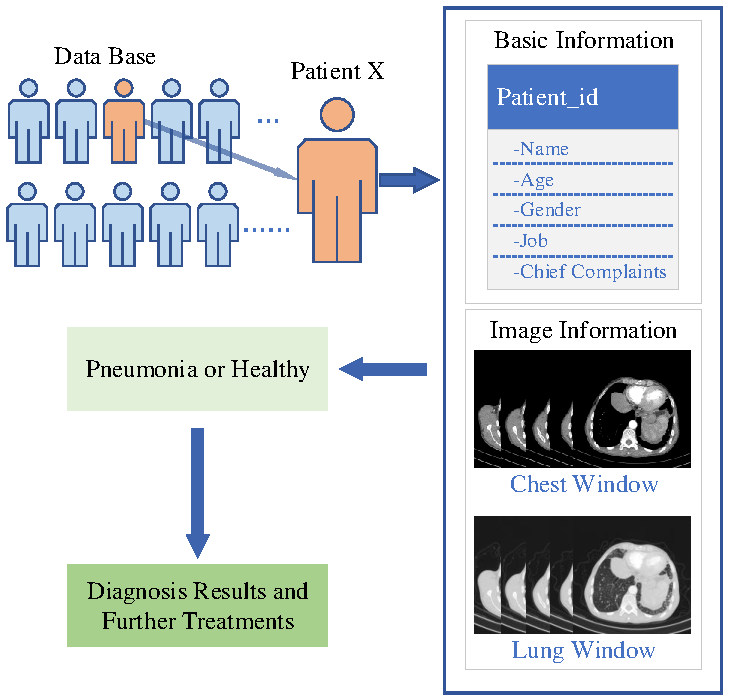
\includegraphics[width=80mm]{clinicalprocess.pdf}}
    \vspace{-0cm}
    \caption{Clinical process of pneumonia screening. The patients' information is kept in data base PACS (Picture Archiving and Communication Systems). Each patient case contains patient basic information like age, gender, name, chief compilations and so on. Meanwhile, image information like CT is kept in PACS with corresponding id. A radiologist needs to consider multi-modal information and refers to images under different windows to give out screening or diagnosing results.}
    \vspace{-0cm}
    \label{clinicalprocess}
    \end{figure}


To address such drawbacks, we propose a novel deep regression framework for pneumonia screening to jointly learn the multi-channel image slices and multimodal clinical, demographic information. Moreover, our framework treats CT slices as short video frames so that we can keep 3D spatial information and reduce the need for calculation resources at the same time.



Fig~\ref{Illustration} illustrates schematic diagram of our framework.
Herein, (a) each CT image will be transformed into a multi-channel image with three windows: Lung Window(LW), High Attenuation(HA) and Low Attenuation(LA). LW provides visual features of normal lung tissues, HA provides visual features of abnormal increase in lung density, LA provides visual features of abnormal decrease in lung density. Three channels complement each other, which not only maintains the ability to extract information from normal lung tissues but also increases the ability to extract information from abnormal lung tissues. All slices will be transformed in sequences and analyzed by a RCNN (Recurrent Convolutional Neural Network).
(b) We also include clinical data in our framework. Chief complaints can provide the location of pain, symptoms, and how long have patients been ill. This information is related to the CT image and enhances the visual features extracted from CT. 
(c) Demographic information about age and gender can provide prior information since patients of different ages and genders have differences in the morphology of the thoracic cavity and lungs. 
(d) The RCNN captures visual features from each multi-channel slices in sequences. An other LSTM is used to analyze semantics from chief complaints. Demographic information will be used as confounding factors. 

\subsection{Contributions}
The main contributions of this work are as follows.

i) We formulate the clinical pneumonia detection process as a regression problem. The proposed framework, which simulates the clinical diagnosing process, takes advantage of the multi-channel images, multi-modal information and avoids the shortcomings of a single source of information.

ii) We propose to treat chest CT scans as short video frames and analyze them using Recurrent Convolutional Neural Network (RCNN). RCNN can make the most of CT image information and reduce the need for calculation resources. Meanwhile, we verify that ResNet50 performs the best when it is combined in RCNN.

iii) We demonstrate that different channels of images can provide different density information during the learning process and help to improve the detection accuracy. We further propose that clinical and demographic information can enhance visual features and provide prior information.

iv) We demonstrate experimentally good performance on a large clinical dataset collected from the First Affiliated Hospital of Army Medical University with 1002 cases.


\section{Evaluation Datasets}
\label{dataset}
\begin{table}[htbp]
    \vspace{-0cm}
    \caption{}
    \vspace{-0cm}
    \begin{center}
    \begin{tabular}{c|c|c|c|c}
    \multicolumn{5}{c}{\textbf{Number of Male and Female Patients in HC and PC}} \\
    \hline
    \textbf{\textit{}} & \textbf{\textit{Healthy}} & \textbf{\textit{pneumonia}}& \textbf{\textit{Total}}& \textbf{\textit{Percentage*}} \\
    \hline
    Male & 240 & 361 & 601 & 60.1\%\\
    Female & 210 & 191 & 401 &47.6\% \\
    \hline
    \textbf{\textit{Total}} & 450 & 552 & 1002 & 55.1\% \\
    
    \hline
    \multicolumn{5}{c}{}\\
    \multicolumn{5}{c}{\textbf{Number of HC and PC in Different Ages}} \\

    \hline
    \textbf{\textit{}} & \textbf{\textit{Healthy}} & \textbf{\textit{pneumonia}}& \textbf{\textit{Total}}& \textbf{\textit{Percentage*}} \\
    \hline
    0-10 & 6 & 1 & 7 & 14.3\%\\
    10-20 & 31 & 2 & 33 & 6.1\%\\
    20-30 & 122 & 30 & 152 & 19.7\%\\
    30-40 & 124 & 45 & 169 &26.6\%\\
    40-50 & 109 & 108 & 217 &49.8\%\\
    50-60 & 53 & 131 & 184 &71.2\%\\
    60-70 & 5 & 126 & 131 &96.2\%\\
    70-80 & 0 & 82 & 82 &100\%\\
    $>90$& 0 & 27 & 27 &100\%\\
    \hline 
    \textbf{\textit{Total}} & 450 & 552 & 1002 & 55.1\% \\

    \hline
    \end{tabular}
    \vspace{0.1cm}
 \\
    \footnotesize{Percentage* is Percentage of Pneumonia Patients. }

    \end{center}
    \label{malefemale}

    \vspace{-0.0cm}
    \end{table}
There have been many datasets for thoracic disease research, but datasets contains CT, demographic and clinical information are rare.
To evaluate our framework, we use the raw data collected from the Radiology Department of The First Affiliated Hospital of Army Medical University. In this study, we have 552 pneumonia cases and 450 healthy cases (1002 cases total) from hospital PACS (Picture Archiving and Communication Systems) in the last three years (2016 - 2019). We show in Table~\ref{malefemale} the details of this dataset. 

Raw data from the hospital may have more than one series of images, and each series has specific data types, image windows, or view angles. 
Generally speaking, radiologists and doctors will use the series under lung window with the smallest `Slice Thickness', but for deep learning models, each case can only have one series. So we design a protocol to pick up specific series for us:

(a) We choose the series with the specific `Convolution Kernel'. Different `Convolution Kernel' indicate different image windows. We need to notice that these names of `Convolution Kernel' vary between hospitals and CT equipment. In our study, we choose `B31f', `I31f 3', `B70f', `B80f', `B70s'. We notice that in the Radiology Department of The First Affiliated Hospital of Army Medical University, `B70s' is the most common parameter used in clinical which contains 620 cases.

(b) We remove series like `Patient Protocol', `Topogram'. These series contain some basic parameters and information about CT equipment, which are not suitable for deep learning.

(c) We calculate `Slice Thickness' of each series, and keep the series with the smallest `Slice Thickness', since small thickness may keep more detailed information about body structure. 

(d) If there were more than one series meet the last two requirements, we would keep the series with the largest number of slices, which could have a larger span of view.

As a result, 552 pneumonia cases and 450 healthy cases (1002 cases total) are left. Since our data are collected from the Radiology Department, the proportion of pneumonia are higher than normal proportion.

The dataset is divided into training / validating / testing sets as 60\% / 20\% / 20\% and make them identically distributed in three parts of datasets, so we have 602 cases in the training set, 200 cases in the validation set, 200 cases in the test set.
Each CT scan has a case file. In case files, we can get patient basic information: patient ID, gender, age, and chief complaints. 

\section{Deep Regression Framework for Pneumonia Detection}
\label{framework}

\subsection{Overview}
\begin{figure*}[htbp]
    \centerline{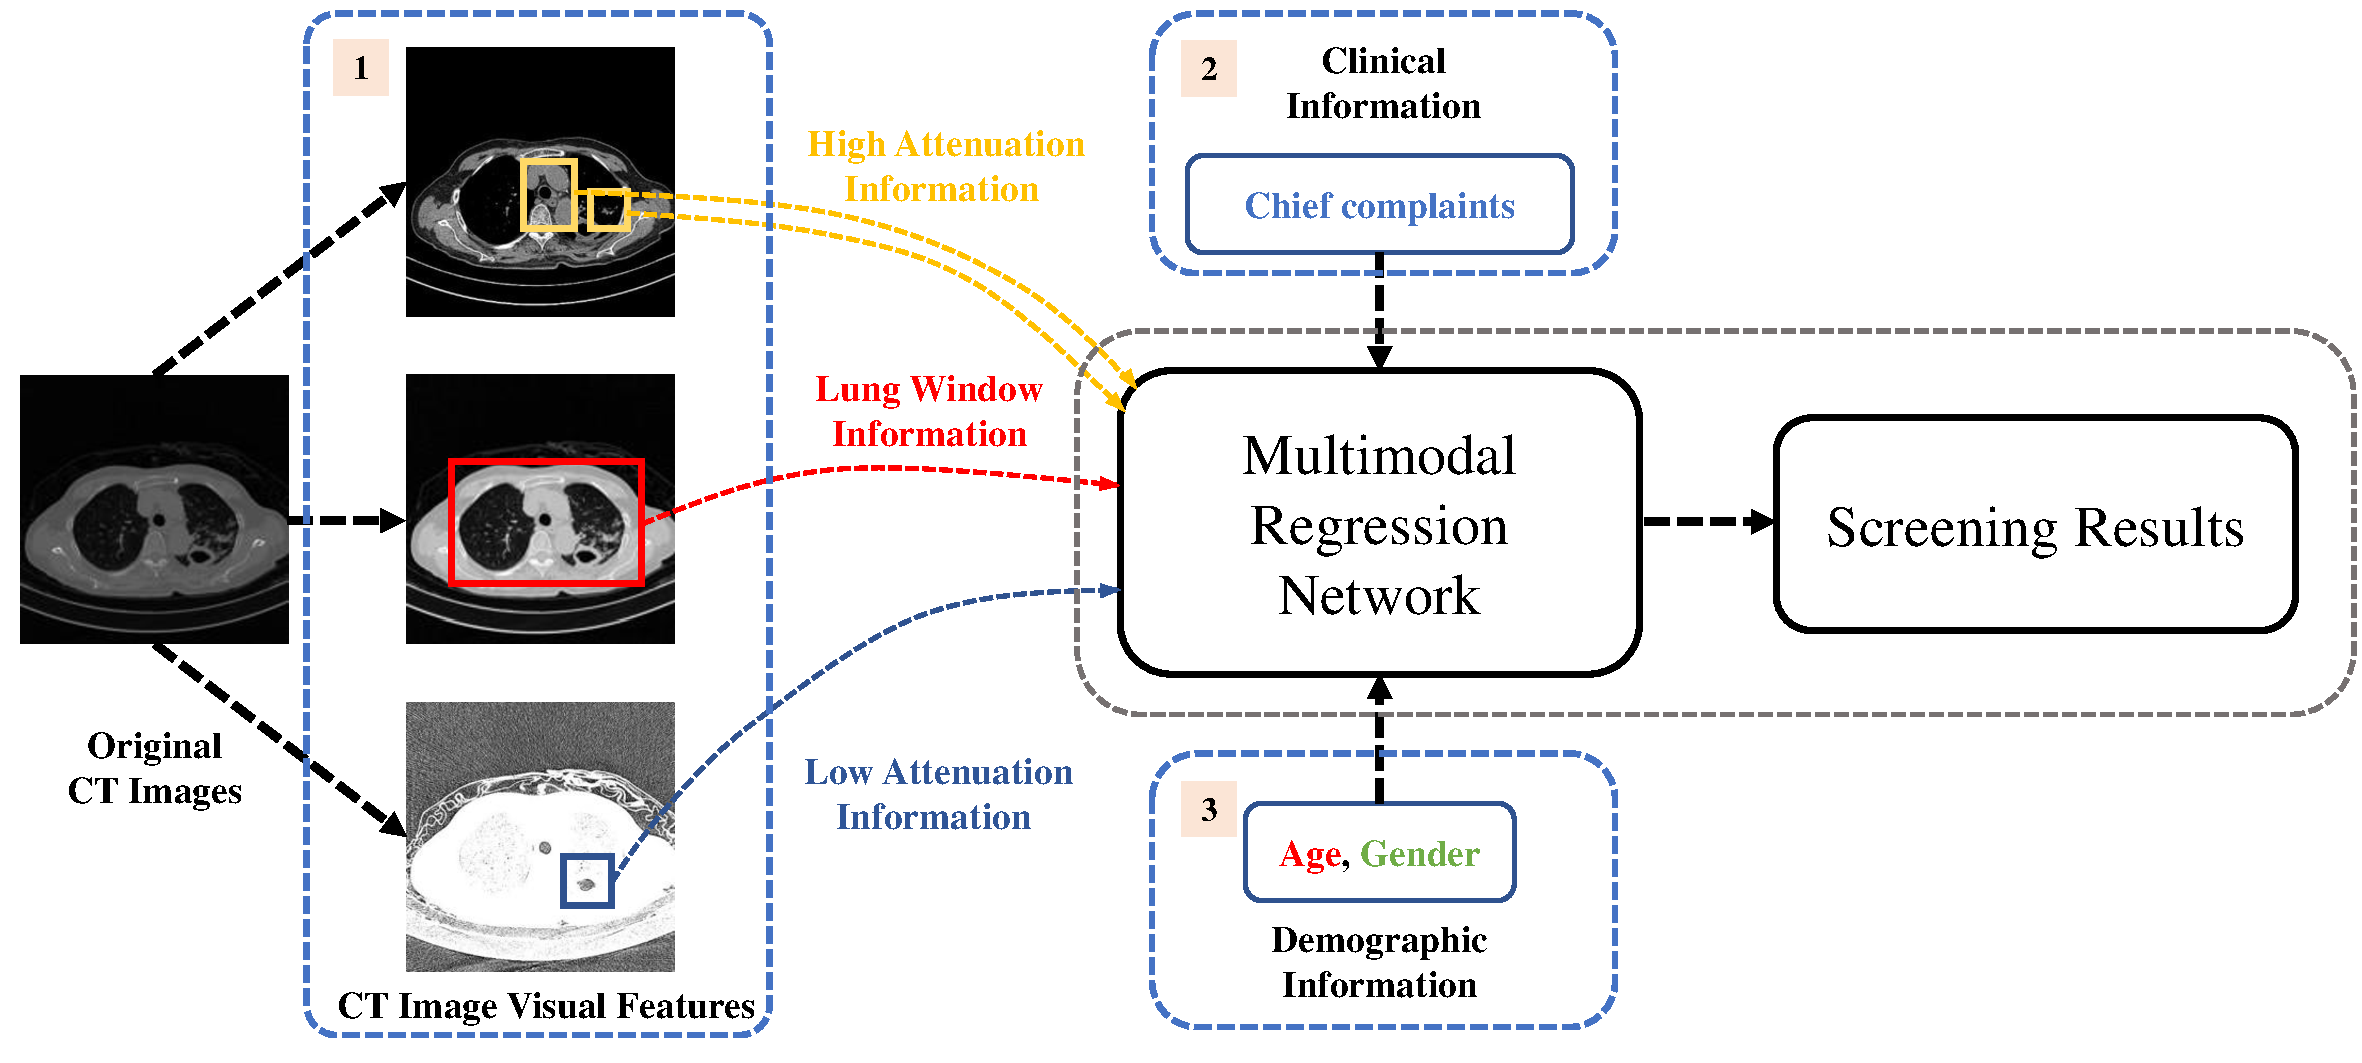
\includegraphics[width=140mm]{new1.pdf}}
    \vspace{-0cm}
    \caption{Illustration of the proposed deep regression framework via multi-channel multi-modal learning for pneumonia detection.
    The inputs of this models are three-channel CT images, clinical chief complaints and demographic information. A RCNN (Recurrent Convolutional Neural Network) is used to capture the visual features. A LSTM is used to analyse chief complaints. Visual features, chief complaints and demographic information will be fed into a deep regression network.}
    \vspace{-0cm}
    \label{Illustration}

    \end{figure*}
The proposed framework, with a schematic illustration shown in Fig~\ref{Illustration}, can be described as a multi-channel multi-modal learning framework. This framework can be regarded as a regression model for classification. All cases will be classified into two Categories: pneumonia cases and healthy cases. As shown in Fig~\ref{Illustration}, there are three kinds of inputs: (1)multi-channel images, (2) clinical information, (3) demographic information. Multi-channel images have three image windows. High Attenuation Window can provide high density information of lungs, Low Attenuation Window can provide low density information, Lung Window can provide general lung information. The regression progress can be formulated as:
\begin{align*}
    P(X) = Softmax(F(V(X) \otimes C(X) \otimes A(X) \otimes G(X)))
\end{align*}
$X$ is the input case, $\otimes$ is the concatenation operation, $V(X)$ is visual features captured from multi-channel images, $C(X)$ is semantic information captured from clinical chief compilations.
$A(X)$ and $G(X)$ indicate patient age and gender. $F$ is a function to fit the regression model of $V(X)$, $C(X)$, $A(X)$ and $G(X)$. $P(X)$ characterizes the likelihood of being pneumonic.

In our framework, a RCNN is used to learn multi-channel CT images and get $V(X)$, a LSTM is used to learn semantics of clinical chief complaints.
Following studies like \cite{dukart2011age, de2016machine}, we treat the demographic information (i.e., age and gender) as confounding factors.

\subsection{Recurrent Convolutional Neural Network}
RCNN (Recurrent Convolutional Neural Network) has been proved to be very effective in video caption, description, and classification \cite{Donahue2015Long, Aafaq2019Spatio}, some studies have applied RCNN to medical image analysis. Majd Zreik et al. \cite{Zreik2018A} recently used RCNN for automatic detection and classification of coronary artery plaque, they used CNN extracts features out of $ 25\times25\times25$ voxels cubes and used an RNN to process the entire sequence using gated recurrent units (GRUs)\cite{chung2014empirical}. KL Tseng et al. \cite{tseng2017joint} exploited convolutional LSTM to model a sequence of 2D slices, and jointly learn the multi-modalities and convolutional LSTM in an end-to-end manner to segment 3D biomedical images.

As mentioned in section~\ref{motiandcont}, CT allows visualization of lung structures, which brings a large amount of redundant information, like muscle, vessels, and bones. It will cost lots of calculation resource if we use 3D CNN directly. However, if we treat CT slices as short video frames, we can analyze them using RCNN instead. In RCNN, each slice will be fed into CNN in sequence and get a sequence of visual features. Then this sequence of features will be fed into RNN, so that we can reduce the need for calculation resource and keep 3D spatial information at the same time. 
This RCNN is actually a encoder for visual features from CT mulit-channel slices.
$V$ mentioned above can be calculated as:
\begin{equation}
    V_t = LSTM(Fx_t, V_{t-1}, z_{t-1})
\end{equation}
$Fx_t$ is the $t$-th visual features in CT slices, $V_{t-1}$ is LSTM hidden state of $t-1$ step, $z_{t-1}$ is LSTM output of $t-1$ step. $t$ is the current step of LSTM. In this study, each scan has 32 steps.

\subsubsection{Convolutional Neural Network}
In this study, we use ResNet50 in RCNN. We compare three kinds of classic CNN models: VGG16 \cite{simonyan2015very}, ResNet \cite{he2016deep} and GoogLeNet with Inception-V3 \cite{szegedy2016rethinking} and our experiments demonstrate that ResNet50 performs the best. This part of experiments will be discussed later in section~\ref{experiments}. We use CNN without fully-connected layers as a feature extractor. We use ResNet50 without fully-connected layers as a feature extractor. The input size of CNN is $512 \times 512$.

\subsubsection{Global Average Pooling}
Since the input size of CNN is $512 \times 512$, the outputs of CNN will be extensive. We use the global average pooling \cite{lin2014network} to reduce the number of neurons significantly. It is a replacement of fully-connected layers to enable the summing of spatial information of feature maps. After global average pooling, we insert a fully-connected layer to reduce dimensions to $128$ to fit the number of LSTM units.

\subsubsection{Long Short-Term Memory}
Recurrent neural networks (RNNs) \cite{bengio1994learning} are a rich class of dynamic models that have been used to generate sequences in domains as diverse as text and motion capture data.
There have been severl kinds of RNN units like GRU \cite{cho2014learning} and LSTM.
In this study, we use LSTM as our RNN cells cause LSTM has been demonstrated to be capable of large-scale learning of sequence data. 

\subsection{Multi-Channel Images Representation}
There are different kinds of image windows for CT reader, such as windows for bone, brain, chest, or lung. Images under different image windows will highlight different tissues of bodies.
As mentioned in section\ref{motiandcont}, each series of CT has one specific `Convolution Kernel'. But it may make data inconsistent between different cases. So we transform raw data into HU(Hounsfield Unit) values. The Hounsfield Unit is a quantitative scale for describing radio-density. After transformed into HU value matrices, all slices form CT scans will have the same unit of measure.

Following the study in \cite{shin2016deep, gao2018holistic}, HU value matrices will be transformed into images using different HU windows. Let $X$ denote the mulit-channel image input, then $X$ can be calculated as:
\begin{align*}
    X=\sum_{q\in\chi}Threshold_{q}[Min, Max]
\end{align*}
$\chi=\{LW, HA, LA\}$, where LW is Lung Window, HA is High Attenuation Window, LA is Low Attenuation Window. $Threshold$ is a threshod method, $Min$ and $Max$ indicate upper and lower limits of HU values. Each image window has corresponding $Min$ and $Max$. Our threshods are hand crafted and little different from studies \cite{shin2016deep, gao2018holistic}:
\begin{align*}
    LW&=Threshold_{LW}[-1000, 400HU]\\
    HA&=Threshold_{HA}[-160, 240HU]\\
    LA&=Threshold_{LA}[-1400, -950HU]\\
\end{align*}

For each slice, it will generate three one-channel grays-cale images. Then we add three one-channel grayscale images into one three-channel false-color RGB image. The `Slice Thickness' between each slice is adjusted into 10mm, and each case will keep 32 slices.
\begin{figure}[htbp]
    \centerline{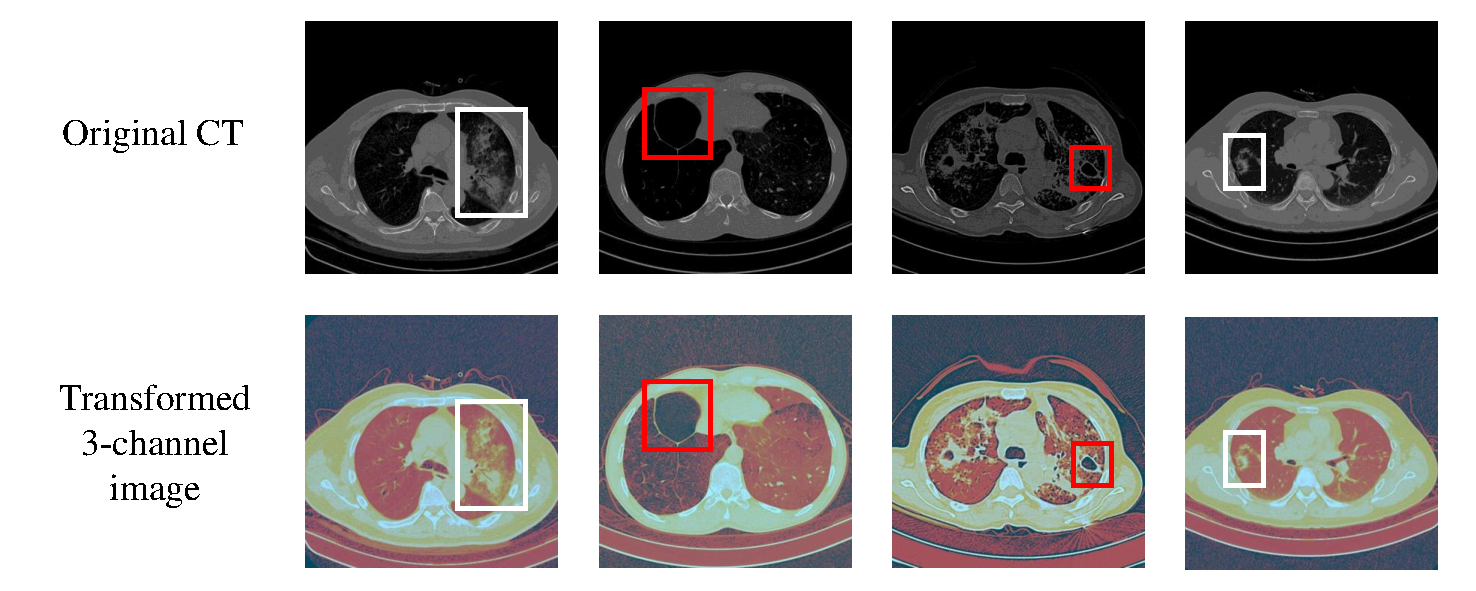
\includegraphics[width=90mm]{3channel2.pdf}}
    \vspace{-0cm}
    \caption{Examples of three-channel images. In this figure, void space (in red rectangle) in original CT images is not very obvious since other normal tissues are in black too. But in the three-channel images, we notice the differences between normal tissues and low dense tissues. Moreover, the details of high dense tissues (in the white rectangle) are still kept in three-channel images.}
    \vspace{-0cm}
    \label{3channel}

    \end{figure}
As shown in Fig~\ref{3channel}, three-channel images can show more information about lung density. Original CT images are grayscale images; high dense tissues are white; normal lung tissues and low dense tissues tend to be black. 
Relatively, three-channel false-color images have a larger scale of colors. First of all, high dense tissues will still tend to be white, like bones, high dense tissues in the lungs. Second, normal lung tissues will tend to be red, and low dense tissues tend to be black, which is very useful when patients have severe lung diseases.

\subsection{Multi-Modal Information Representation}
Studies like \cite{dukart2011age, de2016machine} treated the demographic information as confounding factors. The main disadvantage of such a strategy is that the original representations of subjects will be modified because this strategy adds up several steps of engineered pre-processing in a directed and engineered way. Intuitively, it could further promote the learning performance by adding up demographic information in CAD systems \cite{liu2018joint}.
Following these studies, we also treat demographic information as confounding factors. The demographic information of all studied patients is listed in Table~\ref{malefemale}.

For patients' chief complaints, since all chief complaints are written in Chinese, we have to do Chinese word segmentation. Chinese word segmentation is a challenging problem, so we will take a short cut and use a mature tool: Jieba text segmentation $\footnote[1]{https://github.com/fxsjy/jieba}$ to segment Chinese sentences into Chinese word sequences.

After word segmentation, we use word2vec \cite{mikolov2013efficient, mikolov2013distributed} to embed word sequences into vectors and use CBOW(Continuous Bag-of-Words) to capture relationship between words. Since our corpus is very small, the embedding size is set to $50$, and the window size for CBOW is set to $3$. We set length of Chinese word sequence to $16$ since $16$ is the maximum length among all chief complaint sequences. For those sequences whose length is less than $16$, we add `None' to fill up the voids and increase the length to $16$. Then the sequences will be fed into LSTM:
\begin{equation}
    C_{ct} = LSTM(Word_{ct}, C_{ct-1}, z_{ct-1})
    \label{hct}
\end{equation}
$Word_{ct}$ is word embedding matrix of the $ct$-th word in chief complaint, $C_{ct-1}$ is LSTM hidden state of $ct-1$ step. $ct$ is the current step of this LSTM. 

\subsection{Ensemble of Decisions}
\begin{figure*}[htbp]
    \centerline{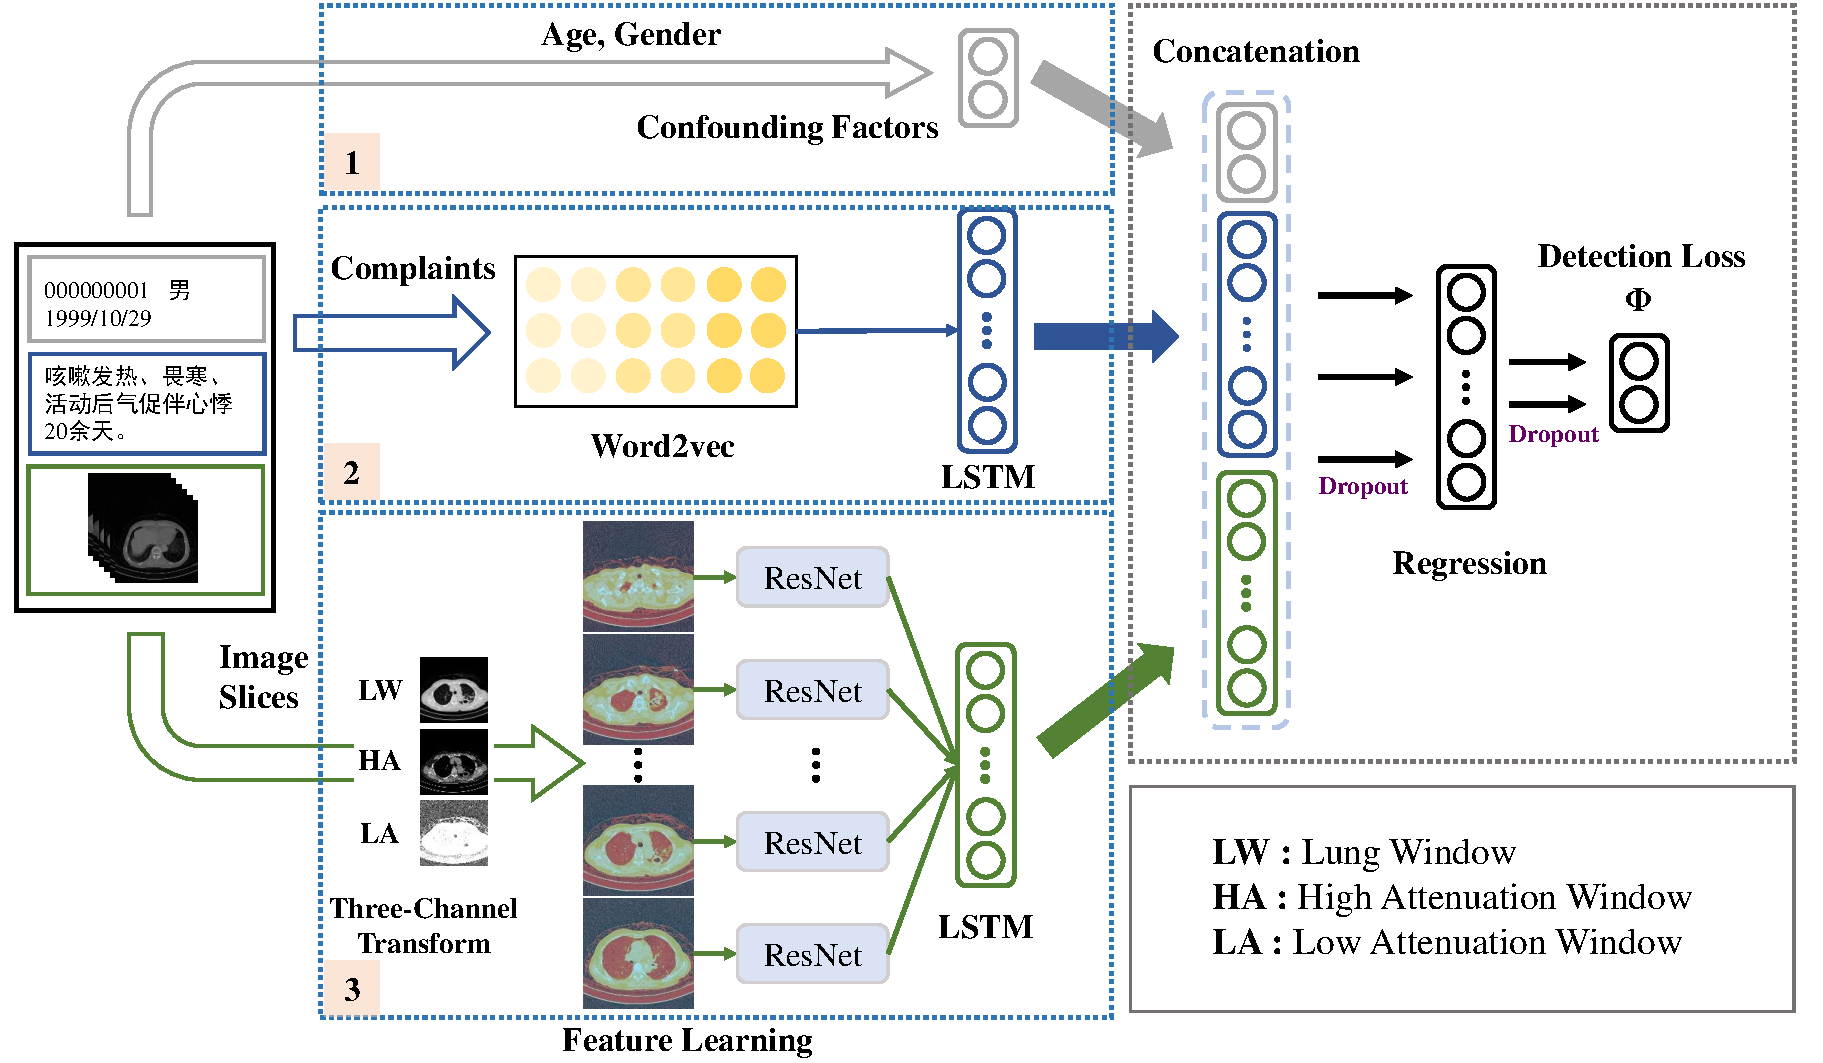
\includegraphics[width=160mm]{MPD2.pdf}}
    \vspace{-0cm}
    \caption{Overview of the deep regression framework via multi-channel mulit-modal learning for pneumonia screening. 
    The black box in the left indicates raw inputs from the hospital.The grey rectangle contains demographic information about age and gender; the blue rectangle contains chief complaints; the green rectangle provides CT image data. Chief complaints will be transformed into matrices by Word2vec and analyze by one LSTM network. Images will be fed into RCNN. Age and gender will be treated as two confounding factors. These three kinds of information will be concatenated and fed into the regression model to simulate the clinical process.}
    \vspace{-0cm}
    \label{architecture}

    \end{figure*}
The over architecture of our framework is shown in Fig~\ref{architecture}.
All information will be fed into a regression model to calculate the likelihood $P$.
We use cross-entropy function as loss function of our model:
\begin{align*}\label{classifyandloss1}
    \mathop{\arg\min}_{W} -\frac{1}{Q} \sum_{q=1}^{Q} \frac{1}{N} \sum_{X_n\in\chi} 1 \{ y_n^q = q\} log(P(y_n^q=q|X_n;W)
\end{align*}
$\chi=\{X_n\}_{n=1}^N$ denotes the training set, $X_n$ represents $n$-th case of training set. $y^q$ are vectors for labels. In this study, the class labels are used in a back-propagation procedure to update the network weights in the convolutional layers, LSTM units, and learn the most relevant features in the fully-connected layers. $W$ denotes the parameters of the model. $Q$ is equal to $2$, which indicates two classes in our data.

\section{Experiments}
\label{experiments}

\subsection{Experimental Setup}
The dataset is divided into training set, validating set and testing set. 602 cases are used to train the framework. Validating and testing sets each has 200 cases. Three sets have the same data distribution.

Source code for data pre-processing and the proposed framework will be released very soon. We will also release the model with trained parameters and some sample cases. But we cannot release dataset because of the privacy of patients. 

\subsection{Parameters}
The initial learning rate is set to 0.0005 and drops 50\% every 3000 training steps. The dropout rate in fully-connected layers is set to 0.5. Our framework will be trained for four epoch, and each epoch contains 15 iterations for all training data. Moreover, we use CNN models pre-trained on ImageNet \cite{ILSVRC15}. Experiments demonstrate that using pre-trained models can significantly improve the converging speed. In this work, all the experiments are run on a GPU of NVIDIA Tesla V100. Each experiment needs about 12G of GPU memory.


\subsection{Baseline System}
To mainifest the advantages offered by the proposed framework, we constructed a baseline framework for compartion: RCNN trained with lung window CT images. 
Generally speaking, we should have a 3D CNN as our baseline. However, the input size is so large that it is impossble to train a 3D CNN under our existing conditions.

We alse developed and repeated the experiments with different RCNN since different CNN models may have impacts on the performance of RCNN. We test three different classic CNN models: ResNet50, VGG16 and GoogLeNet with Inception-V3. We choose the RCNN with the best performance as our baseline system.

\begin{table*}[htbp]    
    \caption{Comparison of All Kinds of RCNN}

    \begin{center}
    \begin{tabular}{c|c|c|c|c|c}

    \hline
    \textbf{\textit{Structure}} & \textbf{\textit{Input Channel}}& \textbf{\textit{Validation Accuracy}} & \textbf{\textit{Validation AUROC}}& \textbf{\textit{Test Accuracy}} & \textbf{\textit{Test AUROC}}\\
    \hline
    RCNN(VGG) & Three Channels& 0.895 &0.894 & 0.845 & 0.841\\
    RCNN(GoogLeNet)& Three Channels & {\bfseries 0.930} & {\bfseries 0.932} & 0.900 & 0.902\\
    RCNN(ResNet) & Three Channels& {\bfseries 0.930} & 0.929 & {\bfseries 0.915} & {\bfseries 0.914}\\
    RCNN(ResNet) & Lung Window & 0.925 & 0.920 & 0.895 & 0.891 \\
    RCNN(ResNet) & Low Attenuation & 0.875 & 0.877 & 0.785 & 0.784 \\
    RCNN(ResNet) & High Attenuation & 0.910 & 0.915 & 0.860 & 0.864 \\

    \hline

    \end{tabular}
    \vspace{-0cm}

    \end{center}
    \vspace{-0cm}\    
    \label{rcnncompare}
    \end{table*}

\subsection{Analyze of Multi-Channel Images}
\label{multianalyze}
In this section, we demonstrate the impacts of mulit-channel images. To remove the impact of clinical and demographic information, the experiments in this section will be carried on RNN models with different CNNs.

We test three kinds of classic CNN models: VGG16 \cite{simonyan2015very}, ResNet \cite{he2016deep} and GoogLeNet with Inception-V3 \cite{szegedy2016rethinking}. Table~\ref{rcnncompare} provides a comprehensive performance comparison on the validating and testing set with different conbination of RCNNs and input channels.

As can be seen in Table~\ref{rcnncompare}, three-channel images can provide more complete visual information of lungs, and RCNN(ResNet) trained with three-channel images have the best performances compared to RCNN(ResNet) models trained with LW, HA, and LA images.
According to experimental results, RCNN(ResNet) trained with lung window images performs the best in three kinds of image windows, which agrees with the clinical practice. As mentioned in section~\ref{dataset}, lung window (i.e., `B70s') is the most common image window in clinical practice. 

Taken alone, low attenuation images and high attenuation images cannot provide enough visual features for RCNN. But when three channels are combined, RCNN achieves the best performance, which means low attenuation images and high attenuation images provide supplementary information for lung window images. It also agrees with clinical practice, since radiologists need to change image windows and look for details if they need to deal with cases with severe diseases.

Moreover, as can be seen in Table~\ref{rcnncompare}, ResNet50 has a better performance on visual features learning than VGG16 and GoogLeNet with Inception-V3. This conclusion is similar to the conclusion drawn in \cite{Wang2017ChestX}, and their experiments showed that ResNet50 outperformed GoogLeNet and VGG16. According to the Table~\ref{rcnncompare}, RCNN(ResNet) and RCNN(GoogLeNet) both achieve 0.930 in validation accuracy, RCNN(GoogLeNet) achieves 0.932 in validatio AUROC, a little better than RCNN(ResNet). However, RCNN(ResNet) has the best performances in both test accuracy and test AUROC. It supports our selection of RCNN(ResNet50) trained with three-channel images as our baseline system.


In order to validate the effect of three-channel images further, we output the feature maps of the convolutional layer, which are displayed in Fig~\ref{show}. More specificity, we output the feature maps after one convolutional layer, one max-pooling layer, and three ResNet blocks, the size of feature maps are $128 \times 128$. To keep experiments environment consistent, all experiments carried on in this part are based on RCNN with ResNet50. Experiments show that CNN trained by three-channel images has advantages over CNNs trained by other kinds of images.

In Fig~\ref{show}, images in the first column are original false-color CT images, which are direct outputs from CT slices. The second, the third and the fourth columns are feature maps from LW CNN, HA CNN, and LA CNN. Images in the last column are feature maps from three-channel CNN.  

According to Fig~\ref{show}, HA window can keep high dense information, but HA has difficulty in capturing the difference between low dense tissues and normal tissues. Contrarily, LA can keep low dense information well, but high dense information tends to be blank in LA. LW window is close to the three-channel window. However, the three-channel window has better discrimination for normal tissues and low dense tissues.
\begin{figure*}[t]
    \centerline{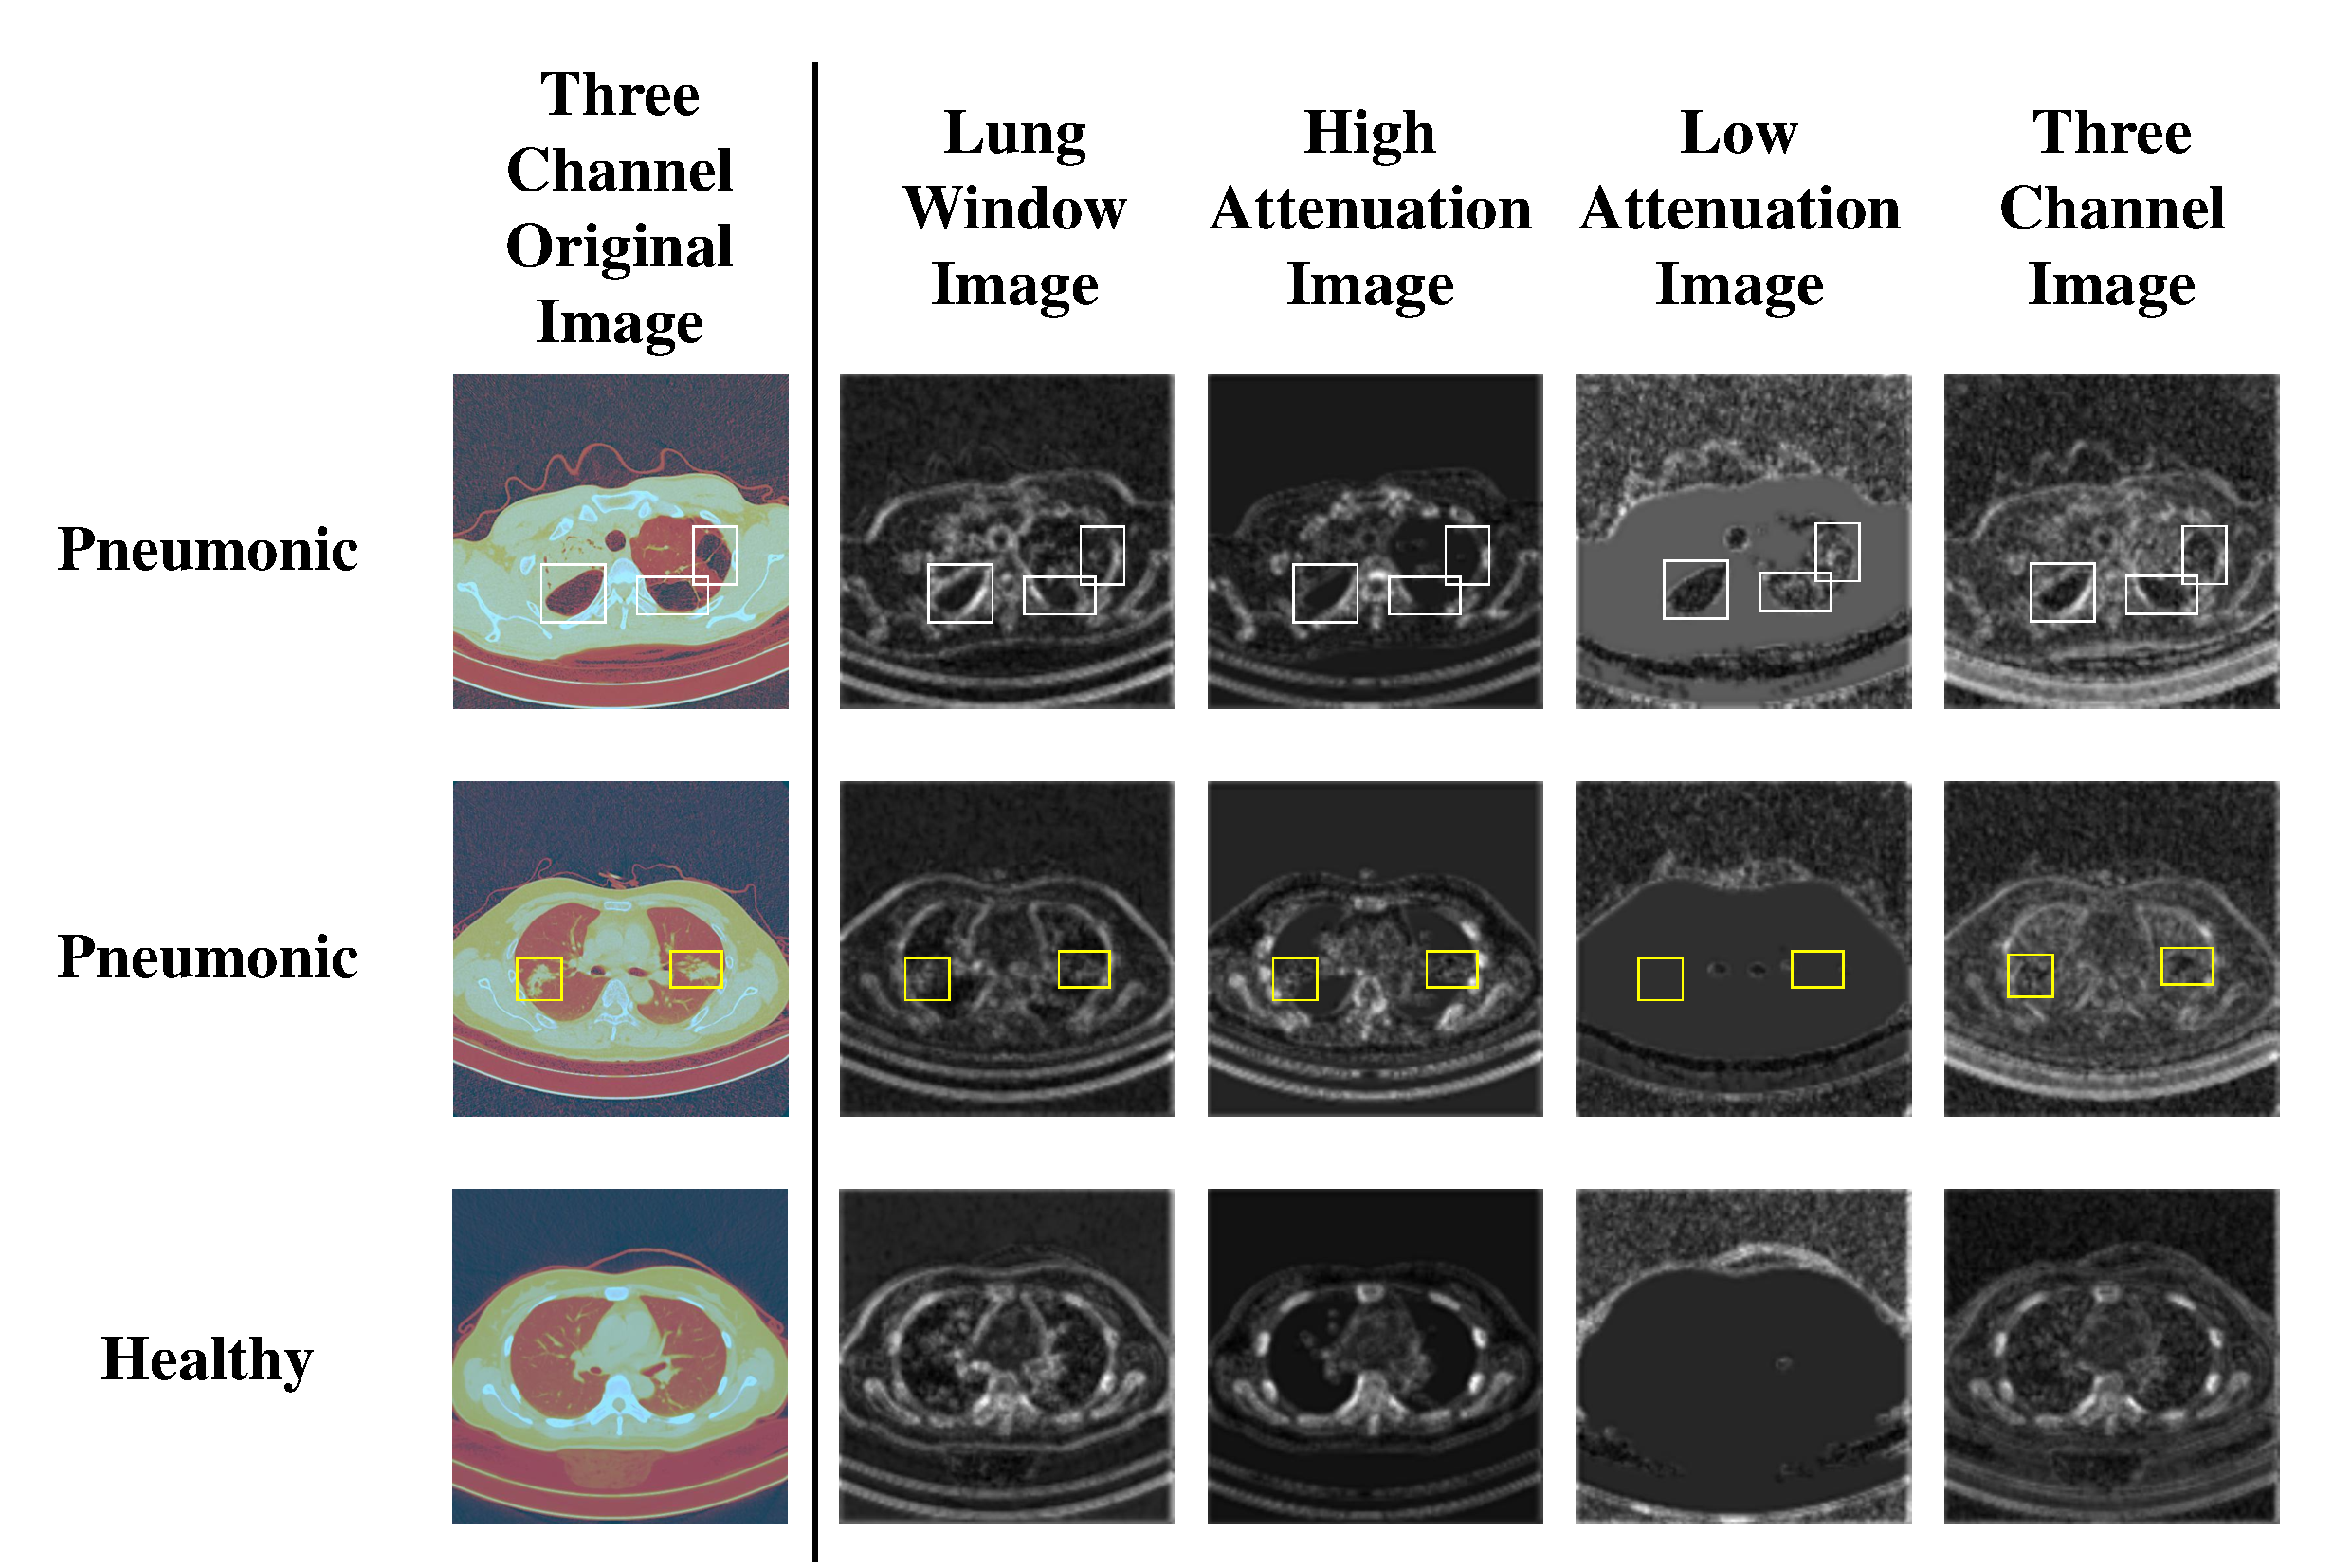
\includegraphics[width=150mm]{show.pdf}}
    \vspace{-0cm}
    \caption{Convolutional Feature Maps from CNN Models Trained by Different Images. 
    The top row shows a pneumonia case which has abnormally low dense areas (white rectangles). The middle row shows a pneumonia case which has abnormal high dense areas (yellow rectangles). During convolutional process, three-channel images can provide both high dense and low dense information. However, low attenuation images can only provide low dense information, high attenuation images can only provide high dense information. Moreover, lung window images have difficulty in distinguishing low dense tissues form normal lung tissues.
    The bottom row is a healthy case. We can compare healthy lung tissues with abnormal low dense tissues and abnormal high dense tissues.
    }
    \vspace{-0cm}
    \label{show}
    \end{figure*}


\subsection{Performance Comparison}
In order to evaluate chief complaints and demographic information separatly, we design two frameworks: one contains all information, the ohter one contains only clinical chief complaints. `RCNN' in this section refers to RCNN(ResNet). 

We show experimental results on testing set in Table~\ref{mpdnetres}. As mentioned in section~\ref{framework}, the output of RCNN, features of clinical and demographic information will be concatenated together and fused by two fully-connected layers. It is simple yet effective. Compared to baseline, clinical chief complaints bring a significant improvements in specificity,but sensitivity will drop to 0.904. This phenomenon indicates that chief complaints can help to classifying healthy cases, but help little in finding pneumonia.

If we add demographic information (i.e., age and gender), the sensitivity will increase to 0.9302, which is the highest in Table~\ref{mpdnetres}. However, the specificity will drop to 0.9298, but still higher than that in RCNN (0.907). 
The accuracy is still 0.930, but the framework has a more balance performance. 
However, in clinical practice, sensitivity is a more important indicator, so that we consider the framework trained with both clinical and demographic information has better clinical performances. 

Moreover, we compare our method with studies in \cite{Wang2017ChestX,yao2017learning, Rajpurkar2017CheXNet, Wang2018TieNet}. Noted that these studies conducted experiments on chest X-Ray images, which is different from the data we use. Table~\ref{mpdnetres} shows that TieNet \cite{Wang2018TieNet} achieved an AUROC of 0.969, which is the highest among these studies. However, this AUROC was achieved by analyzing X-Ray images and reports written by radiologists. If they use images only, the AUROC will drop to 0.658, which indicates that reports provided very string information which is related to pneumonia. We believe it is because the reports written by radiologists contain some conclusions and diagnose results. Using reports to classify images is not quite convincing since radiologists have done the job. Actually in \cite{Wang2018TieNet}, reports only can achieve 0.947, which is much higher than X-Ray images. This pneumonia conforms our assumption.


\begin{table*}[t]
    \caption{Performances of RCNN and the Proposed Framework in Validating Set}
    \begin{center}
    \begin{tabular}{c|c|c|c|c|c}
    \hline
    \textbf{\textit{Structure}} & \textbf{\textit{Data}}& \textbf{\textit{Accuracy}}  & \textbf{\textit{Sensitivity}} & \textbf{\textit{Specificity}} & \textbf{\textit{AUROC}}\\
    \hline
    Wang et al. \cite{Wang2017ChestX}& Chest X-Ray Image & -& - & - & 0.633\\
    Yao et al. \cite{yao2017learning}&Chest X-Ray Image & -& - & - & 0.713\\
    Rajpurkar et al. \cite{Rajpurkar2017CheXNet}&Chest X-Ray Image & -& - & - & 0.768\\
    Wang et al. \cite{Wang2018TieNet} & Chest X-Ray Image \& Report & -& - & - & 0.969\\
    Wang et al. \cite{Wang2018TieNet} & Chest X-Ray & -& - & - & 0.658\\
    Wang et al. \cite{Wang2018TieNet} & Report & -& - & - & 0.947\\

    \hline
    Baseline & Lung Window Image&  0.895 & 0.921 &  0.860 &  0.891 \\
    This Work & Three-Channel Image&  0.915 & 0.921 &  0.907 &  0.914 \\
    This Work & Three-Channel Image \& Complaint &  0.930 & 0.904 &  0.965 & 0.934 \\
    This Work & TC Image \& Complaint \& Age \& Gender&   0.930 & 0.9302 &  0.9298 & 0.925 \\
    \hline
    \end{tabular}
    \vspace{-0cm}
    \end{center}
    \footnotesize{TC indicates Three-Channel Images. Clinical and Demographic Information indicates clinical chief complaints, age and gender.}

    \vspace{-0cm}
    \label{mpdnetres}
    \end{table*}


We further report the confusion matrices of all experiments on validating set in Fig~\ref{Confusionmatrices} so that we can comprehensive compare the impacts of multi-channel images and mulit-modal information. 
We have 200 cases in testing set. Among these cases, 114 cases are pneumonia, the rest are healthy cases. 
The framework trained with multi-channel multi-modal data detects 106 pneumonia cases correctly, higher than ohter models. RCNN(ResNet) trained with three-channel images detects 105 cases of pneumonia, 78 healthy cases. The framework trained with clinical information (i.e., chief complaints) detects 83 healthy cases correctly, which is the best among all models, but its performance in screening pneumonia cases is worse than the framework trained with multi-channel multi-modal data and RCNN(ResNet). 

Four important points should be noticed from the Fig~\ref{Confusionmatrices}.
Firstly, lung window images are able to cope with normal situations in clinical practice. 92.5\% cases can be classified correctly using lung window images.
Secondly, high attenuation window are second choice since normal pneumonia tends to cause increased lung density and high attenuation window can keep these features well. 
Thirdly, the low attenuation window is special, because abnormal decrease in lung density is rare. Only a few patients have such severe pneumonia that cause abnormal decrease in lung density. In spite of the small number, we still have to consider this situation. Framework trained with low attenuation images only performs the worst among three kinds of image windows. However, it can provide necessary supplementary information about low density information.
Fourthly, clinical chief complaints and demographic information further improve the performance of the proposed framework.


\begin{figure*}[htbp]
    \centerline{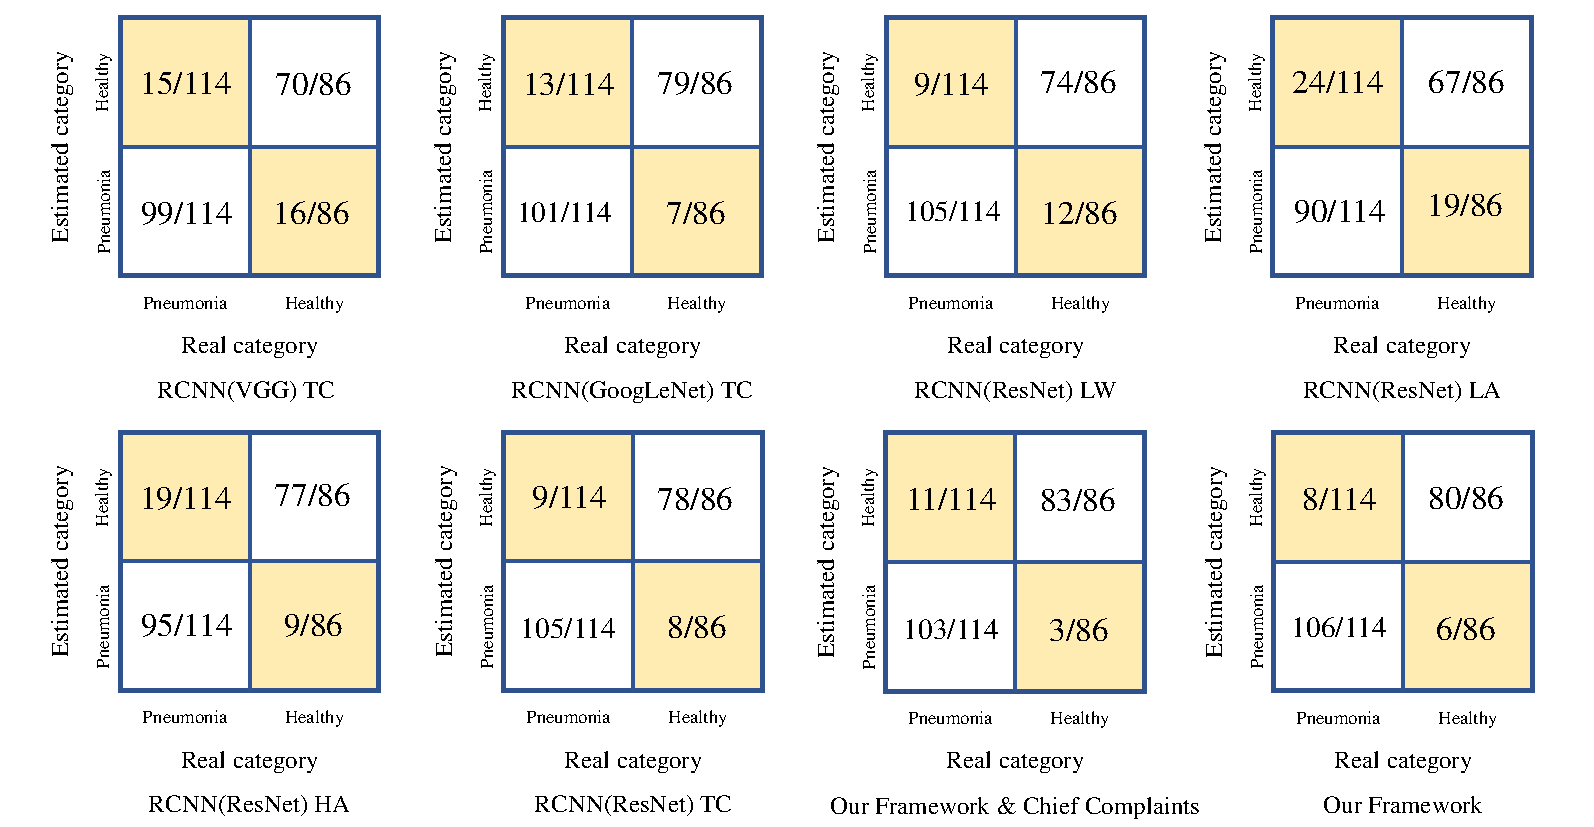
\includegraphics[width=160mm]{Confusionmatrices.pdf}}
    \vspace{-0cm}
    \caption{Confusion matrices achieved by eight different methods in in detection results. We have 144 pneumonia cases and 86 healthy cases in validation set. LW: Lung Window Image, HA: High Attenuation Image, LA: Low Attenuation Image, TC: Three-Channel Image}
    \vspace{-0cm}
    \label{Confusionmatrices}

    \end{figure*}

The validation loss and accuracy during training is shown in Fig~\ref{loss}. According to this figure, the performances in validation accuracy of three models are almost the same. However, the losses of the framework and the framework \& Chief Complaints drop more quickly than RCNN(ResNet), which means clinical and demographic information accelerates the training process. 

This figure indicates that these models do not have much difference in the training process, additional information like chief complaints, age and gender pushes the performance forward a little in the decision making process. It is a little different from our assumption. We assumed that clinical and demographic information can improve the speed of training and performances. But the fact is this additional information only works in the final stage: the decision making stage. This pneumonia indicates that image information is still the most important information resource. Demographic and clinical information can only play a supporting role.

\begin{figure*}[htbp]
    \centerline{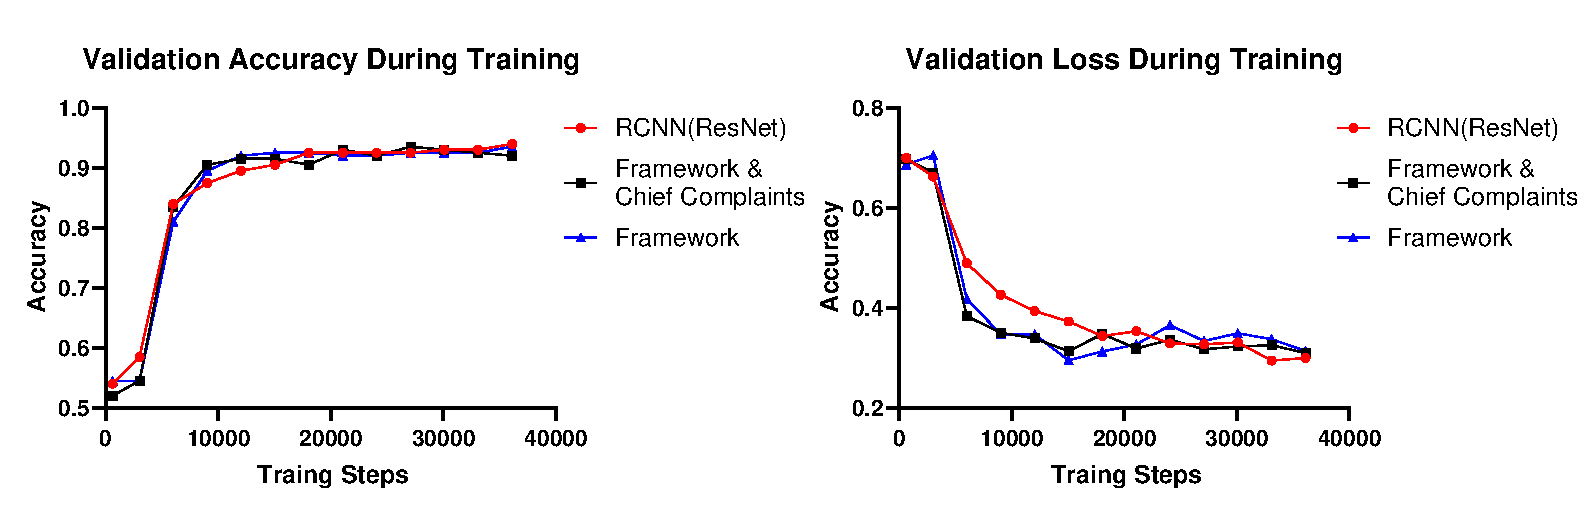
\includegraphics[width=180mm]{aacloss2.pdf}}
    \vspace{-0.5cm}
    \caption{Validation accuracy and loss during training.}
    \vspace{-0cm}
    \label{loss}

    \end{figure*}

\section{Discussion}
\label{discussion}

\subsection{Investigating the Causes of Improvements}
In this section, we demonstrate how the effect of clinical and demographic information imporve the performance of the framework.

To verify that cheif complaints can provide symptoms which are related to pneumonia, we count word frequency about symptoms. Table~\ref{frequency1} shows that the top 10 keywords in HC (healthy cases) and PC (pneumonia cases) have certain regularity. `Cough' is the most frequent keyword in both HC and PC. It appears 256 times (46.4\%) in PC, 183 times (40.7\%) in HC. However, symptoms like `Expectoration', `Fever', `Coughing blood' appear more frequently in PC. For example, `Coughing blood' appears 47 times in PC, but only appears one time in HC. 
\begin{table*}[htb]
    \vspace{-0cm}
\caption{}
\vspace{-0cm}
\begin{center}
\begin{tabular}{c|c|c|c|c}
\multicolumn{5}{c}{\textbf{Top 10 Frequent Key Words in pneumonia Cases}} \\
\hline
    \textbf{\textit{Key Words}} & \textbf{\textit{Frequency in PC}} & \textbf{\textit{Percentage}}& \textbf{\textit{Frequency in HC}}& \textbf{\textit{Percentage}} \\
\hline
\begin{CJK}{UTF8}{gbsn}\textbf{咳嗽}\end{CJK}, \textbf{Cough} & 256 & 0.464 & 183 & 0.407\\
\begin{CJK}{UTF8}{gbsn}\textbf{咳痰}\end{CJK}, \textbf{Expectoration} & 103 & 0.187 & 42 & 0.093\\
\begin{CJK}{UTF8}{gbsn}\textbf{反复}\end{CJK}, \textbf{Repeat Condition} & 65 & 0.118 & 48 & 0.107\\
\begin{CJK}{UTF8}{gbsn}\textbf{气促}\end{CJK}, \textbf{Shortness of Breath} & 60 & 0.109 & 17 & 0.038\\
\begin{CJK}{UTF8}{gbsn}发热\end{CJK}, Fever & 51 & 0.092 & 14 & 0.031\\
\begin{CJK}{UTF8}{gbsn}咯血\end{CJK}, Coughing Blood & 47 & 0.085 & 1 & 0.002\\
\begin{CJK}{UTF8}{gbsn}加重\end{CJK}, Aggravation & 46 & 0.081 & 13 & 0.029\\
\begin{CJK}{UTF8}{gbsn}\textbf{痰}\end{CJK}, \textbf{Sputum} & 32 & 0.058 & 19 & 0.042\\
\begin{CJK}{UTF8}{gbsn}乏力\end{CJK}, Weak& 29 & 0.053 & 7 & 0.016\\
\begin{CJK}{UTF8}{gbsn}感染\end{CJK}, Infection& 28 & 0.051 & 1 & 0.002\\


\hline
\multicolumn{5}{c}{}\\
\multicolumn{5}{c}{\textbf{Top 10 Frequent Key Words in Healthy Cases}} \\
        \hline
        \textbf{\textit{Key Words}} & \textbf{\textit{Frequency in HC}} & \textbf{\textit{Percentage}}& \textbf{\textit{Frequency in PC}}& \textbf{\textit{Percentage}} \\
    \hline
    \begin{CJK}{UTF8}{gbsn}\textbf{咳嗽}\end{CJK}, \textbf{Cough},  & 183 & 0.407 & 256 & 0.464\\
    \begin{CJK}{UTF8}{gbsn}胸痛\end{CJK}, Chest Pain & 67 & 0.149 & 17 & 0.031\\
    \begin{CJK}{UTF8}{gbsn}不适\end{CJK}, Unconfortable & 54 & 0.120 & 25 & 0.045\\
    \begin{CJK}{UTF8}{gbsn}疼痛\end{CJK}, Pain & 53 & 0.118 & 25 & 0.045\\
    \begin{CJK}{UTF8}{gbsn}\textbf{反复}\end{CJK}, \textbf{Repeat Condition} & 48 & 0.107 & 65 & 0.118\\
    \begin{CJK}{UTF8}{gbsn}\textbf{咳痰}\end{CJK}, \textbf{Expectoration} & 42 & 0.093 & 103 & 0.187\\
    \begin{CJK}{UTF8}{gbsn}背痛\end{CJK}, Backache & 28 & 0.062 & 8 & 0.014\\
    \begin{CJK}{UTF8}{gbsn}\textbf{痰}\end{CJK}, \textbf{Sputum}& 19 & 0.042 & 32 & 0.058\\
    \begin{CJK}{UTF8}{gbsn}胸闷\end{CJK}, Chest Tightness & 19 & 0.042 & 16 & 0.029\\
    \begin{CJK}{UTF8}{gbsn}\textbf{气促}\end{CJK}, \textbf{Shortness of Breath}& 17 & 0.038 & 60 & 0.109\\
    
    \hline

\end{tabular}
\vspace{0cm}
\\

\end{center}
\footnotesize{Percentage is frequency divided by number of cases. PC is pneumonia Cases. HC is Healthy Cases. \\
Key words in bold are both top 10 key words in healthy and pneumonia cases.}
\label{frequency1}

\vspace{-0cm}
\end{table*}


According to Table~\ref{frequency1}, patient who have symptoms like expectoration, repeat condition, shortness of breath have larger chance of having pneumonia. Patients who have chest pain, or feel unconfortable have less chance of having pneumonia. Having cough, on the other hand, is a symptom with minimal discrimination.

Moreover, we count the number of words which can provide information of location. In 1002 cases, every 2 cases contain 1 words which can help to locate the lesions (appear 504 times). 
Fig~\ref{txtpic} shows two examples. According to the location and symptom information provided by chief complaints, we can accurately locate lesions in CT. 

In Fig~\ref{txtpic}, words marked red is information related to location, words marked blue are related to symptoms. In the first case, its chief complaint locates the symptoms in the right lower lung, and then we find shadows in the accurate place. In the second case, it chief complaint says that this patient has pains in right chest, then we also find shadows in the right lung in CT images.
This phenomenon demonstrates that information from chief complaints is related to CT images, and can assist deep learning model.    

Then we further demonstrate the effect of demographic information. As mentioned before, demographic information can provide prior information. According to the Table~\ref{malefemale} mentioned above, we observe some interesting patterns:

(i) A male patient has a more significant chance of getting pneumonia. In 601 male cases, about 60\% of them are pneumonia; however, in 401 female cases, only 47.6\% are pneumonia. This phenomenon may be related to smoking since males in Chinese suffer a severe smoking problem; 

(2) The table shows that age is also associated with the chance of getting pneumonia. We can observe that people older than 40 have a much larger chance of getting pneumonia. There are about half of healthy cases between 40-50, but this indication drops so quickly that it goes down to 28.8\% between 50-60. 

\begin{figure}[t]
    \centerline{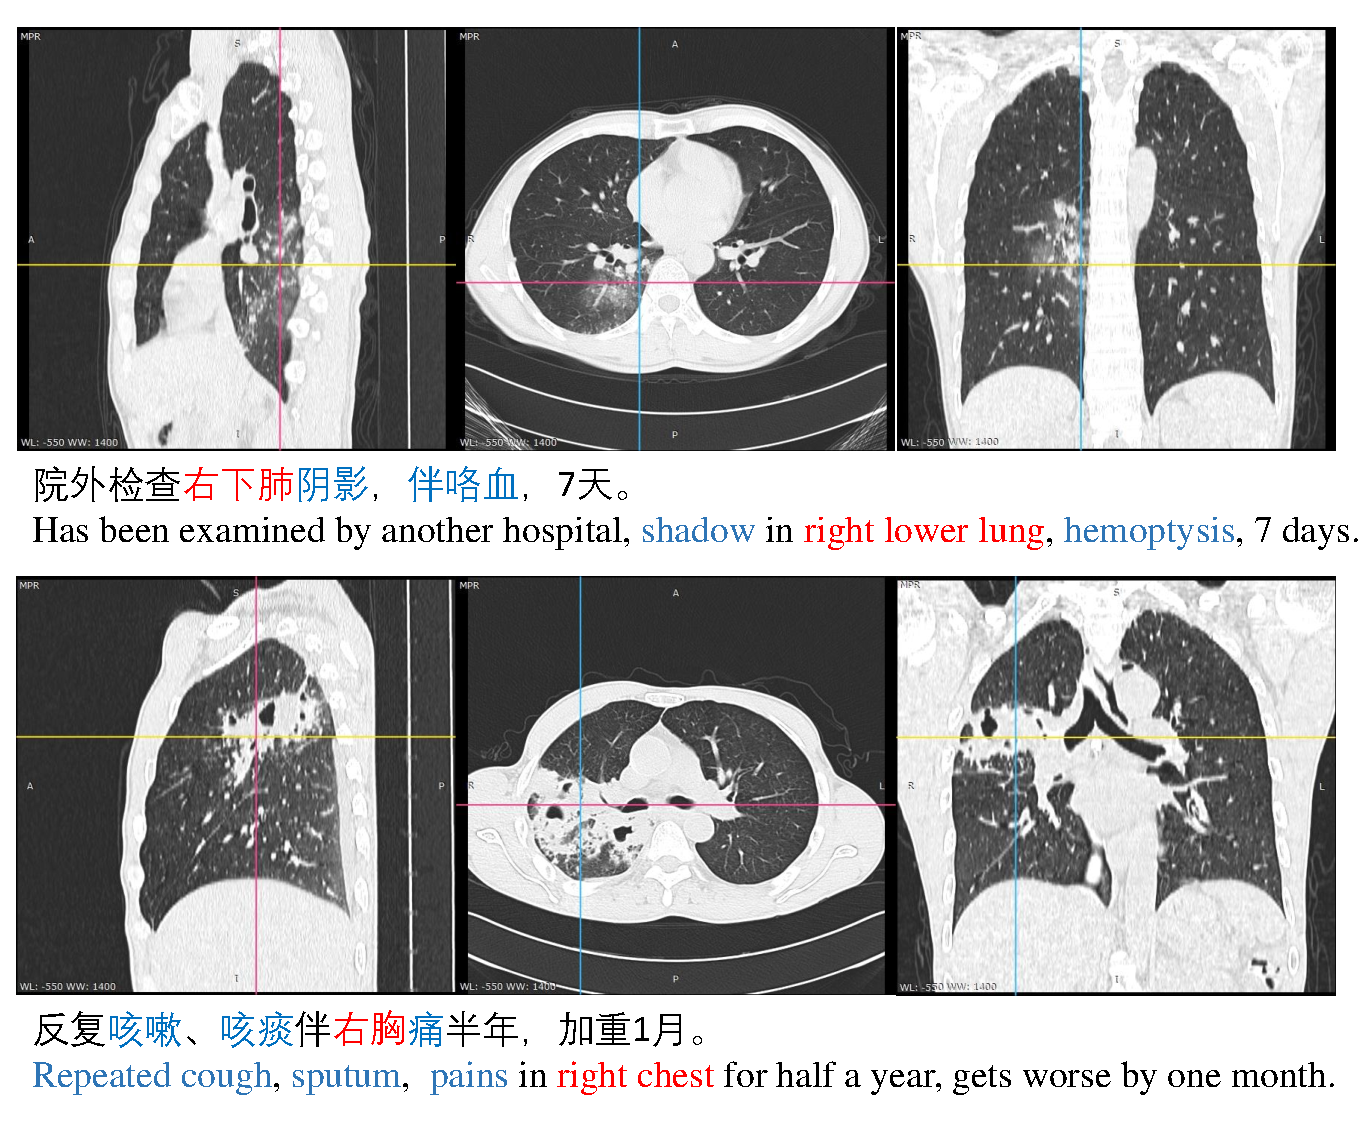
\includegraphics[width=85mm]{txtpic.pdf}}
    \vspace{-0cm}
    \caption{Chief complaints can provide information related to CT images. In this figure, we show two pneumonia cases, and each case has chief complaints provided by patients. Words marked red give the location, and words marked blue provide symptoms. English chief complaints are translated from Chinese above. Location and symptoms information provided by chief complaints are related to abnormal tissues in CT images.}
    \vspace{-0cm}
    \label{txtpic}
    \end{figure}


According to these two patterns, we can clearly observe that demographic information can provide a strong prior information. These two kinds of demographic information will be treated as confounding factors and help to imporve the performance of the whole framework.

\subsection{Limitations and Future Work}
Even if our framework can screen pneumonia using multimodal data, there are still some shortcomings in our work.

Firstly, we analyze 1002 cases in this study. But 1002 cases are far small than `big data', so our model's performance is restricted by data distribution and quality. 

Secondly, we only consider chest CT scans, chief complaints, gender, and age. In clinical practice, besides the tests mentioned above, patients usually need to take blood pressure measurements, blood tests, heartbeat measurements, and other tests. These examinations can help doctors gain a more objective and comprehensive understanding of the patient condition so that doctors can make a more accurate diagnose.

However, it is very difficult to overcome these two shortcomings mentioned above since data collected from PACS are disorder. Constructing a big scale medical dataset with consistent data is a very challenging task, cause raw data is affected by radiologists' habits, data acquisition equipment, and hospital work rules. 
Our future work will focus on finding a method which can perform accurate diagnose on disorder data and include multimodal information from more medical tests.

\section{Conclusions}
\label{conclusions}
In this study, we propose a novel mulit-channel multi-modal deep regression framework, which combines CT visual features with patients' age, gender, and chief complaints to simulates clinical practice. 
The proposed framework extracts visual features from three-channel images, semantic features from chief complaints, and fuses these features with prior information provided by age and gender.

We analyze 1002 cases (450 healthy cases and 552 pneumonia cases) from the Radiology Department of The First Affiliated Hospital of Army Medical University. Experiments demonstrate that the proposed framework achieves promising performance.


% Can use something like this to put references on a page
% by themselves when using endfloat and the captionsoff option.
\ifCLASSOPTIONcaptionsoff
  \newpage
\fi



% trigger a \newpage just before the given reference
% number - used to balance the columns on the last page
% adjust value as needed - may need to be readjusted if
% the document is modified later
%\IEEEtriggeratref{8}
% The "triggered" command can be changed if desired:
%\IEEEtriggercmd{\enlargethispage{-5in}}

% references section

% can use a bibliography generated by BibTeX as a .bbl file
% BibTeX documentation can be easily obtained at:
% http://mirror.ctan.org/biblio/bibtex/contrib/doc/
% The IEEEtran BibTeX style support page is at:
% http://www.michaelshell.org/tex/thebibliography/bibtex/
\bibliographystyle{IEEEtran}
% argument is your BibTeX string definitions and bibliography database(s)

% reference refs
\bibliography{refs}


%
% <OR> manually copy in the resultant .bbl file
% set second argument of \begin to the number of references
% (used to reserve space for the reference number labels box)





% biography section
% 
% If you have an EPS/PDF photo (graphicx package needed) extra braces are
% needed around the contents of the optional argument to biography to prevent
% the LaTeX parser from getting confused when it sees the complicated
% \includegraphics command within an optional argument. (You could create
% your own custom macro containing the \includegraphics command to make things
% simpler here.)
%\begin{IEEEbiography}[{\includegraphics[width=1in,height=1.25in,clip,keepaspectratio]{mshell}}]{Michael Shell}
% or if you just want to reserve a space for a photo:

% \begin{IEEEbiography}{Michael Shell}
% Biography text here.
% \end{IEEEbiography}

% if you will not have a photo at all:


\newpage

\begin{IEEEbiography}[{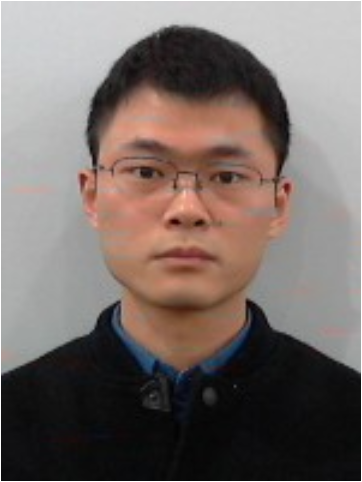
\includegraphics[width=1in,height=1.25in,clip,keepaspectratio]{qiuliwang.png}}]{Qiuli~Wang}
    received the B.E. degree in the School of Information Engineering, Yangzhou University in 2016. He is currently working toward the Ph.D. degree in the School of Big Data \& Software Engineering, Chongqing University. 
    His research interests include medical image computing, deep learning, so on.
\end{IEEEbiography}

\vspace{-0.5cm}

\begin{IEEEbiography}[{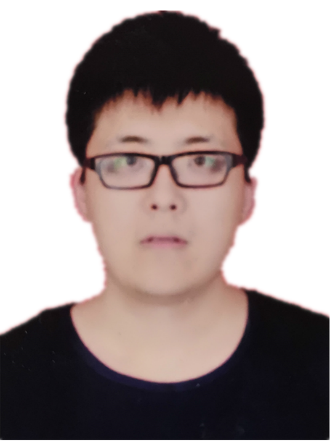
\includegraphics[width=1in,height=1.25in,clip,keepaspectratio]{zhihuanli.png}}]{Zhihuan~Li}
    received the B.E degree in Geological Engineering from China University of Mining and Technology, Xvzhou, China in 2016. He is currently working toward the M.S. degree in Software Engineering from the Department of Big Data \& Software Engineering, Chongqing University, Chongqing.
	His research interests include medical image analysis , segmentation and so on.
\end{IEEEbiography}

\vspace{-0.5cm}
\begin{IEEEbiography}[{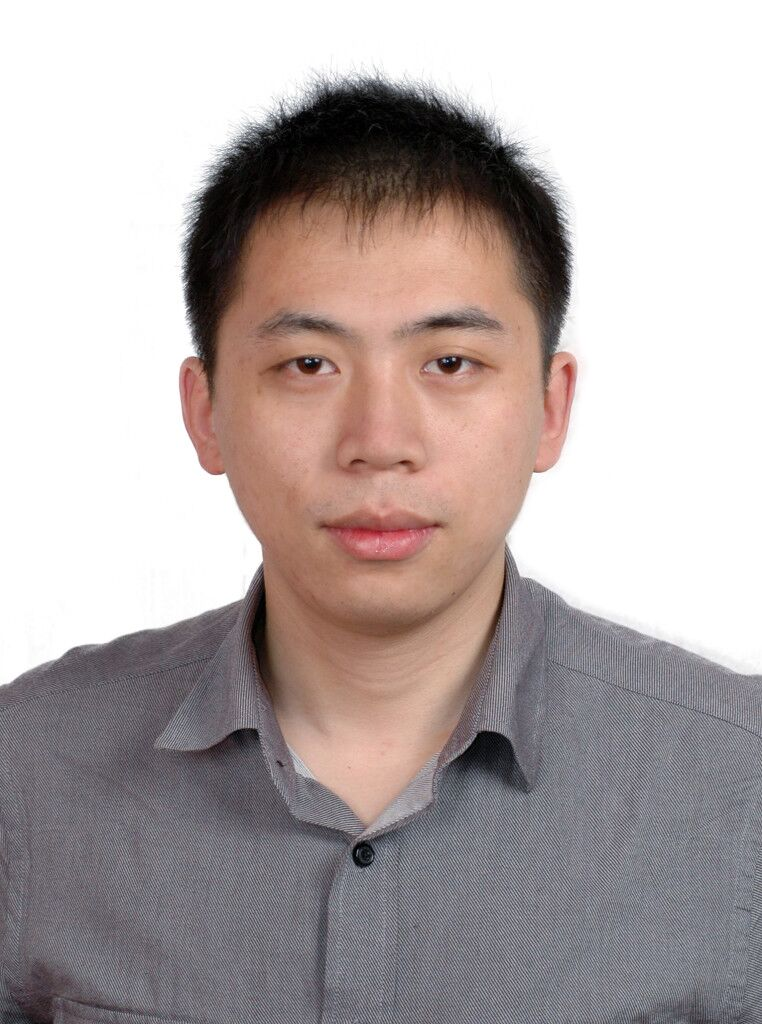
\includegraphics[width=1in,height=1.25in,clip,keepaspectratio]{chenliu.png}}]{Chen~Liu}
    received the M.D. degree in Medical Imaging from Army Medical University, China, in 2015. He is currently an attending physicians in the Radiology Department of Southwest Hospital which is the first affiliated hospital of Army Medical University. He has hosted more than 6 research including National Natural Science Foundation and got funded more than 1.6 million. He published 6 articles as first author. His current research interests include brain functional MRI, clinical data mining, medical imaging deep learning.
\end{IEEEbiography}




\vspace{-0.5cm}

\begin{IEEEbiography}[{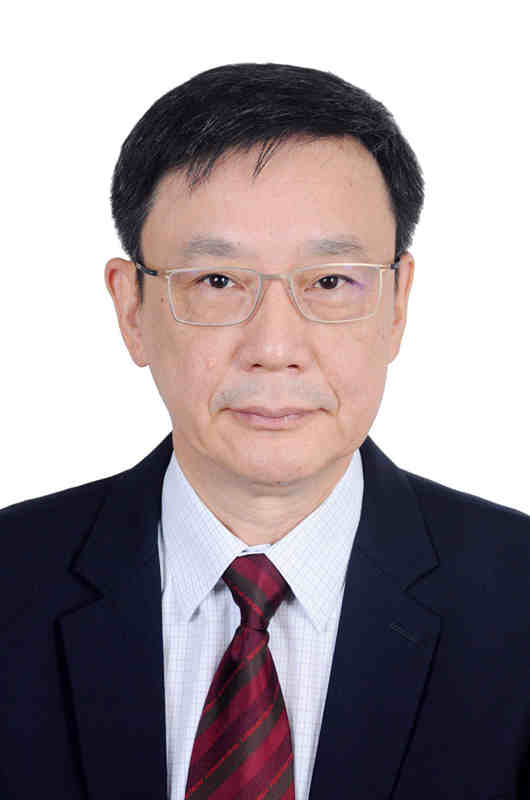
\includegraphics[width=1in,height=1.25in,clip,keepaspectratio]{danyang.png}}]{Dan~Yang}
    received the B.Eng. degree in automation, the M.S. degree in applied mathematics, and the Ph.D. degree in machinery manufacturing and automation from Chongqing University, Chongqing. From 1997 to 1999, he held a post-doctoral position with the University of Electro-Communications, Tokyo, Japan. He is currently the President of Southwest Jiaotong University. He is also a Professor with the School of Big Data \& Software Engineering, Chongqing University. He has authored over 100 scientific papers and some of them are published in some authoritative journals and conferences, such as the IEEE TRANSACTIONS ON PATTERN ANALYSIS AND MACHINE INTELLIGENCE, CVPR, and BMVC. His research interests include computer vision, image processing, pattern recognition, software engineering,
and scientific computing.
\end{IEEEbiography}
\vspace{-0.5cm}

\begin{IEEEbiography}[{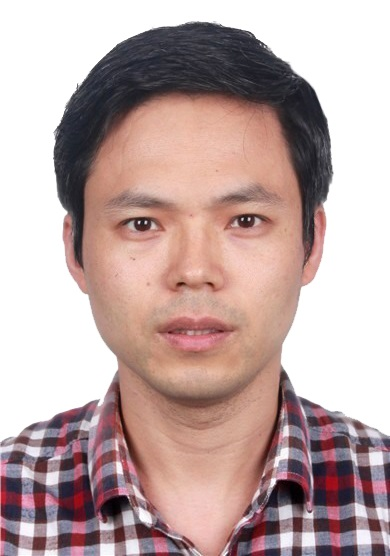
\includegraphics[width=1in,height=1.25in,clip,keepaspectratio]{xiaohongzhang.png}}]{Xiaohong~Zhang}
    received the M.S. degree in applied mathematics from Chongqing University, China, where he also received the Ph.D. degree in computer software and theory, in 2006. He is currently a Professor and the Vice Dean with the School of Big Data \& Software Engineering, Chongqing University. His current research interests include data mining of software engineering, topic modeling, image semantic analysis, and video analysis.
\end{IEEEbiography}
\vspace{-0.5cm}

% insert where needed to balance the two columns on the last page with
% biographies
%\newpage

% \begin{IEEEbiographynophoto}{XXX}
%     XXX
% \end{IEEEbiographynophoto}

% You can push biographies down or up by placing
% a \vfill before or after them. The appropriate
% use of \vfill depends on what kind of text is
% on the last page and whether or not the columns
% are being equalized.

%\vfill

% Can be used to pull up biographies so that the bottom of the last one
% is flush with the other column.
%\enlargethispage{-5in}



% that's all folks
\end{document}


